\documentclass[1p]{elsarticle_modified}
%\bibliographystyle{elsarticle-num}

%\usepackage[colorlinks]{hyperref}
%\usepackage{abbrmath_seonhwa} %\Abb, \Ascr, \Acal ,\Abf, \Afrak
\usepackage{amsfonts}
\usepackage{amssymb}
\usepackage{amsmath}
\usepackage{amsthm}
\usepackage{scalefnt}
\usepackage{amsbsy}
\usepackage{kotex}
\usepackage{caption}
\usepackage{subfig}
\usepackage{color}
\usepackage{graphicx}
\usepackage{xcolor} %% white, black, red, green, blue, cyan, magenta, yellow
\usepackage{float}
\usepackage{setspace}
\usepackage{hyperref}

\usepackage{tikz}
\usetikzlibrary{arrows}

\usepackage{multirow}
\usepackage{array} % fixed length table
\usepackage{hhline}

%%%%%%%%%%%%%%%%%%%%%
\makeatletter
\renewcommand*\env@matrix[1][\arraystretch]{%
	\edef\arraystretch{#1}%
	\hskip -\arraycolsep
	\let\@ifnextchar\new@ifnextchar
	\array{*\c@MaxMatrixCols c}}
\makeatother %https://tex.stackexchange.com/questions/14071/how-can-i-increase-the-line-spacing-in-a-matrix
%%%%%%%%%%%%%%%

\usepackage[normalem]{ulem}

\newcommand{\msout}[1]{\ifmmode\text{\sout{\ensuremath{#1}}}\else\sout{#1}\fi}
%SOURCE: \msout is \stkout macro in https://tex.stackexchange.com/questions/20609/strikeout-in-math-mode

\newcommand{\cancel}[1]{
	\ifmmode
	{\color{red}\msout{#1}}
	\else
	{\color{red}\sout{#1}}
	\fi
}

\newcommand{\add}[1]{
	{\color{blue}\uwave{#1}}
}

\newcommand{\replace}[2]{
	\ifmmode
	{\color{red}\msout{#1}}{\color{blue}\uwave{#2}}
	\else
	{\color{red}\sout{#1}}{\color{blue}\uwave{#2}}
	\fi
}

\newcommand{\Sol}{\mathcal{S}} %segment
\newcommand{\D}{D} %diagram
\newcommand{\A}{\mathcal{A}} %arc


%%%%%%%%%%%%%%%%%%%%%%%%%%%%%5 test

\def\sl{\operatorname{\textup{SL}}(2,\Cbb)}
\def\psl{\operatorname{\textup{PSL}}(2,\Cbb)}
\def\quan{\mkern 1mu \triangleright \mkern 1mu}

\theoremstyle{definition}
\newtheorem{thm}{Theorem}[section]
\newtheorem{prop}[thm]{Proposition}
\newtheorem{lem}[thm]{Lemma}
\newtheorem{ques}[thm]{Question}
\newtheorem{cor}[thm]{Corollary}
\newtheorem{defn}[thm]{Definition}
\newtheorem{exam}[thm]{Example}
\newtheorem{rmk}[thm]{Remark}
\newtheorem{alg}[thm]{Algorithm}

\newcommand{\I}{\sqrt{-1}}
\begin{document}

%\begin{frontmatter}
%
%\title{Boundary parabolic representations of knots up to 8 crossings}
%
%%% Group authors per affiliation:
%\author{Yunhi Cho} 
%\address{Department of Mathematics, University of Seoul, Seoul, Korea}
%\ead{yhcho@uos.ac.kr}
%
%
%\author{Seonhwa Kim} %\fnref{s_kim}}
%\address{Center for Geometry and Physics, Institute for Basic Science, Pohang, 37673, Korea}
%\ead{ryeona17@ibs.re.kr}
%
%\author{Hyuk Kim}
%\address{Department of Mathematical Sciences, Seoul National University, Seoul 08826, Korea}
%\ead{hyukkim@snu.ac.kr}
%
%\author{Seokbeom Yoon}
%\address{Department of Mathematical Sciences, Seoul National University, Seoul, 08826,  Korea}
%\ead{sbyoon15@snu.ac.kr}
%
%\begin{abstract}
%We find all boundary parabolic representation of knots up to 8 crossings.
%
%\end{abstract}
%\begin{keyword}
%    \MSC[2010] 57M25 
%\end{keyword}
%
%\end{frontmatter}

%\linenumbers
%\tableofcontents
%
\newcommand\colored[1]{\textcolor{white}{\rule[-0.35ex]{0.8em}{1.4ex}}\kern-0.8em\color{red} #1}%
%\newcommand\colored[1]{\textcolor{white}{ #1}\kern-2.17ex	\textcolor{white}{ #1}\kern-1.81ex	\textcolor{white}{ #1}\kern-2.15ex\color{red}#1	}

{\Large $\underline{12a_{0435}~(K12a_{0435})}$}

\setlength{\tabcolsep}{10pt}
\renewcommand{\arraystretch}{1.6}
\vspace{1cm}\begin{tabular}{m{100pt}>{\centering\arraybackslash}m{274pt}}
\multirow{5}{120pt}{
	\centering
	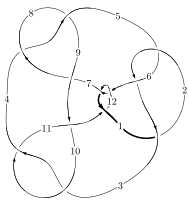
\includegraphics[width=112pt]{../../../GIT/diagram.site/Diagrams/png/1236_12a_0435.png}\\
\ \ \ A knot diagram\footnotemark}&
\allowdisplaybreaks
\textbf{Linearized knot diagam} \\
\cline{2-2}
 &
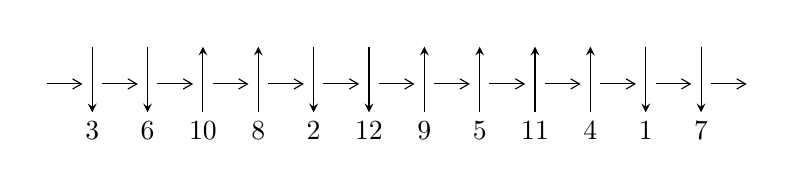
\begin{tikzpicture}[x=20pt, y=17pt]
	% nodes
	\node (C0) at (0, 0) {};
	\node (C1) at (1, 0) {};
	\node (C1U) at (1, +1) {};
	\node (C1D) at (1, -1) {3};

	\node (C2) at (2, 0) {};
	\node (C2U) at (2, +1) {};
	\node (C2D) at (2, -1) {6};

	\node (C3) at (3, 0) {};
	\node (C3U) at (3, +1) {};
	\node (C3D) at (3, -1) {10};

	\node (C4) at (4, 0) {};
	\node (C4U) at (4, +1) {};
	\node (C4D) at (4, -1) {8};

	\node (C5) at (5, 0) {};
	\node (C5U) at (5, +1) {};
	\node (C5D) at (5, -1) {2};

	\node (C6) at (6, 0) {};
	\node (C6U) at (6, +1) {};
	\node (C6D) at (6, -1) {12};

	\node (C7) at (7, 0) {};
	\node (C7U) at (7, +1) {};
	\node (C7D) at (7, -1) {9};

	\node (C8) at (8, 0) {};
	\node (C8U) at (8, +1) {};
	\node (C8D) at (8, -1) {5};

	\node (C9) at (9, 0) {};
	\node (C9U) at (9, +1) {};
	\node (C9D) at (9, -1) {11};

	\node (C10) at (10, 0) {};
	\node (C10U) at (10, +1) {};
	\node (C10D) at (10, -1) {4};

	\node (C11) at (11, 0) {};
	\node (C11U) at (11, +1) {};
	\node (C11D) at (11, -1) {1};

	\node (C12) at (12, 0) {};
	\node (C12U) at (12, +1) {};
	\node (C12D) at (12, -1) {7};
	\node (C13) at (13, 0) {};

	% arrows
	\draw[->,>={angle 60}]
	(C0) edge (C1) (C1) edge (C2) (C2) edge (C3) (C3) edge (C4) (C4) edge (C5) (C5) edge (C6) (C6) edge (C7) (C7) edge (C8) (C8) edge (C9) (C9) edge (C10) (C10) edge (C11) (C11) edge (C12) (C12) edge (C13) ;	\draw[->,>=stealth]
	(C1U) edge (C1D) (C2U) edge (C2D) (C3D) edge (C3U) (C4D) edge (C4U) (C5U) edge (C5D) (C6U) edge (C6D) (C7D) edge (C7U) (C8D) edge (C8U) (C9D) edge (C9U) (C10D) edge (C10U) (C11U) edge (C11D) (C12U) edge (C12D) ;
	\end{tikzpicture} \\
\hhline{~~} \\& 
\textbf{Solving Sequence} \\ \cline{2-2} 
 &
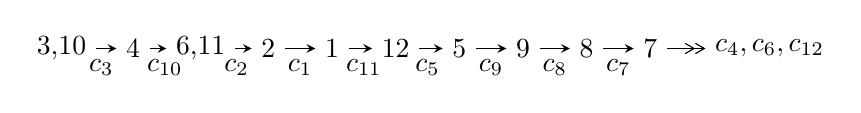
\begin{tikzpicture}[x=23pt, y=7pt]
	% node
	\node (A0) at (-1/8, 0) {3,10};
	\node (A1) at (1, 0) {4};
	\node (A2) at (33/16, 0) {6,11};
	\node (A3) at (25/8, 0) {2};
	\node (A4) at (33/8, 0) {1};
	\node (A5) at (41/8, 0) {12};
	\node (A6) at (49/8, 0) {5};
	\node (A7) at (57/8, 0) {9};
	\node (A8) at (65/8, 0) {8};
	\node (A9) at (73/8, 0) {7};
	\node (C1) at (1/2, -1) {$c_{3}$};
	\node (C2) at (3/2, -1) {$c_{10}$};
	\node (C3) at (21/8, -1) {$c_{2}$};
	\node (C4) at (29/8, -1) {$c_{1}$};
	\node (C5) at (37/8, -1) {$c_{11}$};
	\node (C6) at (45/8, -1) {$c_{5}$};
	\node (C7) at (53/8, -1) {$c_{9}$};
	\node (C8) at (61/8, -1) {$c_{8}$};
	\node (C9) at (69/8, -1) {$c_{7}$};
	\node (A10) at (11, 0) {$c_{4},c_{6},c_{12}$};

	% edge
	\draw[->,>=stealth]	
	(A0) edge (A1) (A1) edge (A2) (A2) edge (A3) (A3) edge (A4) (A4) edge (A5) (A5) edge (A6) (A6) edge (A7) (A7) edge (A8) (A8) edge (A9) ;
	\draw[->>,>={angle 60}]	
	(A9) edge (A10);
\end{tikzpicture} \\ 

\end{tabular} \\

\footnotetext{
The image of knot diagram is generated by the software ``\textbf{Draw programme}" developed by Andrew Bartholomew(\url{http://www.layer8.co.uk/maths/draw/index.htm\#Running-draw}), where we modified some parts for our purpose(\url{https://github.com/CATsTAILs/LinksPainter}).
}\phantom \\ \newline 
\centering \textbf{Ideals for irreducible components\footnotemark of $X_{\text{par}}$} 
 
\begin{align*}
I^u_{1}&=\langle 
-3 u^{21}-10 u^{20}+\cdots+8 b+6,\;6 u^{21}+21 u^{20}+\cdots+8 a-18,\;u^{22}+3 u^{21}+\cdots+2 u+2\rangle \\
I^u_{2}&=\langle 
-10 u^{15} a-44 u^{15}+\cdots+23 a-60,\;-6 u^{15} a-7 u^{15}+\cdots-18 a-1,\\
\phantom{I^u_{2}}&\phantom{= \langle  }u^{16}- u^{15}-3 u^{14}+4 u^{13}+6 u^{12}-9 u^{11}-5 u^{10}+12 u^9+3 u^8-11 u^7+u^6+8 u^5- u^4-5 u^3+3 u^2+2 u-1\rangle \\
I^u_{3}&=\langle 
2494307142 u^{31}+7215726931 u^{30}+\cdots+4328817643 b-18964617036,\\
\phantom{I^u_{3}}&\phantom{= \langle  }4190268217 u^{31}+38131442460 u^{30}+\cdots+60603447002 a-118490829071,\\
\phantom{I^u_{3}}&\phantom{= \langle  }u^{32}+3 u^{31}+\cdots-24 u-7\rangle \\
I^u_{4}&=\langle 
-4001108 u^{23} a-234438 u^{23}+\cdots+6117289 a-712901,\\
\phantom{I^u_{4}}&\phantom{= \langle  }17866 u^{23} a-3017 u^{23}+\cdots+14683 a+59324,\;u^{24}- u^{23}+\cdots-4 u+1\rangle \\
I^u_{5}&=\langle 
-2 a^3+12 a^2+68 b+43 a+47,\;2 a^4+2 a^3+9 a^2-8 a+11,\;u+1\rangle \\
I^u_{6}&=\langle 
b+1,\;u^2+2 a+u,\;u^4- u^2+2\rangle \\
I^u_{7}&=\langle 
-2 a^3+14 a^2+105 b+74 a+69,\;2 a^4+4 a^3+10 a^2+9,\;u-1\rangle \\
I^u_{8}&=\langle 
b-1,\;u^3- u^2+2 a- u-1,\;u^4+1\rangle \\
I^u_{9}&=\langle 
b,\;a+1,\;u-1\rangle \\
I^u_{10}&=\langle 
-2 a u+4 b-2 a+u+5,\;4 a^2-4 a+17,\;u^2+2 u+1\rangle \\
\end{align*}\\
\begin{align*}
I^u_{11}&=\langle 
b+1,\;u+1\rangle \\
\\
I^v_{1}&=\langle 
a,\;b-1,\;v+1\rangle \\
\end{align*}
\raggedright * 11 irreducible components of $\dim_{\mathbb{C}}=0$, with total 156 representations.\\
\raggedright * 1 irreducible components of $\dim_{\mathbb{C}}=1$ \\
\footnotetext{All coefficients of polynomials are rational numbers. But the coefficients are sometimes approximated in decimal forms when there is not enough margin.}
\newpage
\renewcommand{\arraystretch}{1}
\centering \section*{I. $I^u_{1}= \langle -3 u^{21}-10 u^{20}+\cdots+8 b+6,\;6 u^{21}+21 u^{20}+\cdots+8 a-18,\;u^{22}+3 u^{21}+\cdots+2 u+2 \rangle$}
\flushleft \textbf{(i) Arc colorings}\\
\begin{tabular}{m{7pt} m{180pt} m{7pt} m{180pt} }
\flushright $a_{3}=$&$\begin{pmatrix}1\\0\end{pmatrix}$ \\
\flushright $a_{10}=$&$\begin{pmatrix}0\\u\end{pmatrix}$ \\
\flushright $a_{4}=$&$\begin{pmatrix}1\\- u^2\end{pmatrix}$ \\
\flushright $a_{6}=$&$\begin{pmatrix}-\frac{3}{4} u^{21}-\frac{21}{8} u^{20}+\cdots+\frac{15}{4} u+\frac{9}{4}\\\frac{3}{8} u^{21}+\frac{5}{4} u^{20}+\cdots-2 u-\frac{3}{4}\end{pmatrix}$ \\
\flushright $a_{11}=$&$\begin{pmatrix}u\\- u^3+u\end{pmatrix}$ \\
\flushright $a_{2}=$&$\begin{pmatrix}-\frac{5}{4} u^{21}-\frac{33}{8} u^{20}+\cdots+\frac{19}{4} u+\frac{9}{4}\\\frac{5}{8} u^{21}+\frac{5}{2} u^{20}+\cdots-\frac{7}{2} u-\frac{3}{4}\end{pmatrix}$ \\
\flushright $a_{1}=$&$\begin{pmatrix}-\frac{5}{8} u^{21}-\frac{13}{8} u^{20}+\cdots+\frac{5}{4} u+\frac{3}{2}\\\frac{5}{8} u^{21}+\frac{5}{2} u^{20}+\cdots-\frac{7}{2} u-\frac{3}{4}\end{pmatrix}$ \\
\flushright $a_{12}=$&$\begin{pmatrix}\frac{3}{8} u^{20}+\frac{9}{8} u^{19}+\cdots+\frac{3}{4} u-\frac{1}{4}\\-\frac{3}{8} u^{21}-\frac{5}{4} u^{20}+\cdots+2 u+\frac{3}{4}\end{pmatrix}$ \\
\flushright $a_{5}=$&$\begin{pmatrix}\frac{1}{4} u^{20}+\frac{3}{4} u^{19}+\cdots-\frac{1}{2} u+\frac{1}{2}\\-\frac{1}{4} u^{20}-\frac{3}{4} u^{19}+\cdots+\frac{1}{2} u+\frac{1}{2}\end{pmatrix}$ \\
\flushright $a_{9}=$&$\begin{pmatrix}- u^3\\u^5- u^3+u\end{pmatrix}$ \\
\flushright $a_{8}=$&$\begin{pmatrix}-\frac{1}{4} u^{21}-\frac{3}{4} u^{20}+\cdots+\frac{1}{2} u^2-\frac{1}{2} u\\\frac{1}{4} u^{21}+\frac{3}{4} u^{20}+\cdots-\frac{1}{2} u^2+\frac{1}{2} u\end{pmatrix}$ \\
\flushright $a_{7}=$&$\begin{pmatrix}-\frac{1}{4} u^{21}-\frac{3}{4} u^{20}+\cdots+\frac{1}{2} u^2-\frac{1}{2} u\\\frac{1}{4} u^{21}+\frac{3}{4} u^{20}+\cdots-\frac{1}{2} u^2+\frac{1}{2} u\end{pmatrix}$\\&\end{tabular}
\flushleft \textbf{(ii) Obstruction class $= -1$}\\~\\
\flushleft \textbf{(iii) Cusp Shapes $= -\frac{5}{4} u^{21}-\frac{9}{2} u^{20}-6 u^{19}+\frac{13}{4} u^{18}+\frac{41}{2} u^{17}+\frac{61}{4} u^{16}-38 u^{15}-\frac{295}{4} u^{14}+\frac{17}{4} u^{13}+121 u^{12}+\frac{143}{2} u^{11}-\frac{449}{4} u^{10}-\frac{639}{4} u^9+u^8+131 u^7+\frac{319}{4} u^6-\frac{141}{4} u^5-\frac{287}{4} u^4-36 u^3-\frac{3}{2} u^2+16 u+\frac{21}{2}$}\\~\\
\newpage\renewcommand{\arraystretch}{1}
\flushleft \textbf{(iv) u-Polynomials at the component}\newline \\
\begin{tabular}{m{50pt}|m{274pt}}
Crossings & \hspace{64pt}u-Polynomials at each crossing \\
\hline $$\begin{aligned}c_{1},c_{11}\end{aligned}$$&$\begin{aligned}
&u^{22}+9 u^{21}+\cdots+12 u+4
\end{aligned}$\\
\hline $$\begin{aligned}c_{2},c_{5},c_{6}\\c_{12}\end{aligned}$$&$\begin{aligned}
&u^{22}+3 u^{21}+\cdots+2 u+2
\end{aligned}$\\
\hline $$\begin{aligned}c_{3},c_{4},c_{8}\\c_{10}\end{aligned}$$&$\begin{aligned}
&u^{22}-3 u^{21}+\cdots-2 u+2
\end{aligned}$\\
\hline $$\begin{aligned}c_{7},c_{9}\end{aligned}$$&$\begin{aligned}
&u^{22}-9 u^{21}+\cdots-12 u+4
\end{aligned}$\\
\hline
\end{tabular}\\~\\
\newpage\renewcommand{\arraystretch}{1}
\flushleft \textbf{(v) Riley Polynomials at the component}\newline \\
\begin{tabular}{m{50pt}|m{274pt}}
Crossings & \hspace{64pt}Riley Polynomials at each crossing \\
\hline $$\begin{aligned}c_{1},c_{7},c_{9}\\c_{11}\end{aligned}$$&$\begin{aligned}
&y^{22}+15 y^{21}+\cdots-144 y+16
\end{aligned}$\\
\hline $$\begin{aligned}c_{2},c_{3},c_{4}\\c_{5},c_{6},c_{8}\\c_{10},c_{12}\end{aligned}$$&$\begin{aligned}
&y^{22}-9 y^{21}+\cdots-12 y+4
\end{aligned}$\\
\hline
\end{tabular}\\~\\
\newpage\flushleft \textbf{(vi) Complex Volumes and Cusp Shapes}
$$\begin{array}{c|c|c}  
\text{Solutions to }I^u_{1}& \I (\text{vol} + \sqrt{-1}CS) & \text{Cusp shape}\\
 \hline 
\begin{aligned}
u &= -0.460930 + 0.893438 I \\
a &= \phantom{-}0.684435 + 0.437574 I \\
b &= \phantom{-}1.153190 - 0.551408 I\end{aligned}
 & -4.71017 + 7.32959 I & -5.39190 - 4.27146 I \\ \hline\begin{aligned}
u &= -0.460930 - 0.893438 I \\
a &= \phantom{-}0.684435 - 0.437574 I \\
b &= \phantom{-}1.153190 + 0.551408 I\end{aligned}
 & -4.71017 - 7.32959 I & -5.39190 + 4.27146 I \\ \hline\begin{aligned}
u &= \phantom{-}0.988250 + 0.370938 I \\
a &= -1.03648 - 1.21462 I \\
b &= \phantom{-}1.065270 + 0.737606 I\end{aligned}
 & \phantom{-}4.11009 - 3.23667 I & \phantom{-}2.24331 - 1.56003 I \\ \hline\begin{aligned}
u &= \phantom{-}0.988250 - 0.370938 I \\
a &= -1.03648 + 1.21462 I \\
b &= \phantom{-}1.065270 - 0.737606 I\end{aligned}
 & \phantom{-}4.11009 + 3.23667 I & \phantom{-}2.24331 + 1.56003 I \\ \hline\begin{aligned}
u &= -0.784487 + 0.839661 I \\
a &= -0.861171 + 0.910993 I \\
b &= -1.104870 - 0.465097 I\end{aligned}
 & -5.88667 - 8.79084 I & -4.97697 + 9.61140 I \\ \hline\begin{aligned}
u &= -0.784487 - 0.839661 I \\
a &= -0.861171 - 0.910993 I \\
b &= -1.104870 + 0.465097 I\end{aligned}
 & -5.88667 + 8.79084 I & -4.97697 - 9.61140 I \\ \hline\begin{aligned}
u &= \phantom{-}1.104870 + 0.465097 I \\
a &= -0.25047 + 1.91615 I \\
b &= \phantom{-}0.784487 - 0.839661 I\end{aligned}
 & \phantom{-}5.88667 + 8.79084 I & \phantom{-}4.97697 - 9.61140 I \\ \hline\begin{aligned}
u &= \phantom{-}1.104870 - 0.465097 I \\
a &= -0.25047 - 1.91615 I \\
b &= \phantom{-}0.784487 + 0.839661 I\end{aligned}
 & \phantom{-}5.88667 - 8.79084 I & \phantom{-}4.97697 + 9.61140 I \\ \hline\begin{aligned}
u &= \phantom{-}0.969240 + 0.733052 I \\
a &= -0.502789 - 0.521520 I \\
b &= -0.727531 + 0.091585 I\end{aligned}
 & -2.94270 + 5.73222 I & \phantom{-}2.37742 - 7.71227 I \\ \hline\begin{aligned}
u &= \phantom{-}0.969240 - 0.733052 I \\
a &= -0.502789 + 0.521520 I \\
b &= -0.727531 - 0.091585 I\end{aligned}
 & -2.94270 - 5.73222 I & \phantom{-}2.37742 + 7.71227 I\\
 \hline 
 \end{array}$$\newpage$$\begin{array}{c|c|c}  
\text{Solutions to }I^u_{1}& \I (\text{vol} + \sqrt{-1}CS) & \text{Cusp shape}\\
 \hline 
\begin{aligned}
u &= -0.599304 + 0.453735 I \\
a &= \phantom{-}0.368330 - 0.822096 I \\
b &= \phantom{-}0.024798 + 0.642855 I\end{aligned}
 & \phantom{-}0.42065 - 1.46148 I & \phantom{-}2.50513 + 4.69748 I \\ \hline\begin{aligned}
u &= -0.599304 - 0.453735 I \\
a &= \phantom{-}0.368330 + 0.822096 I \\
b &= \phantom{-}0.024798 - 0.642855 I\end{aligned}
 & \phantom{-}0.42065 + 1.46148 I & \phantom{-}2.50513 - 4.69748 I \\ \hline\begin{aligned}
u &= \phantom{-}0.727531 + 0.091585 I \\
a &= \phantom{-}0.96246 - 1.93359 I \\
b &= -0.969240 + 0.733052 I\end{aligned}
 & \phantom{-}2.94270 + 5.73222 I & -2.37742 - 7.71227 I \\ \hline\begin{aligned}
u &= \phantom{-}0.727531 - 0.091585 I \\
a &= \phantom{-}0.96246 + 1.93359 I \\
b &= -0.969240 - 0.733052 I\end{aligned}
 & \phantom{-}2.94270 - 5.73222 I & -2.37742 + 7.71227 I \\ \hline\begin{aligned}
u &= -1.153190 + 0.551408 I \\
a &= -1.09782 + 0.94427 I \\
b &= \phantom{-}0.460930 - 0.893438 I\end{aligned}
 & \phantom{-}4.71017 - 7.32959 I & \phantom{-}5.39190 + 4.27146 I \\ \hline\begin{aligned}
u &= -1.153190 - 0.551408 I \\
a &= -1.09782 - 0.94427 I \\
b &= \phantom{-}0.460930 + 0.893438 I\end{aligned}
 & \phantom{-}4.71017 + 7.32959 I & \phantom{-}5.39190 - 4.27146 I \\ \hline\begin{aligned}
u &= -1.065270 + 0.737606 I \\
a &= -0.072097 + 0.382579 I \\
b &= -0.988250 + 0.370938 I\end{aligned}
 & -4.11009 - 3.23667 I & -2.24331 - 1.56003 I \\ \hline\begin{aligned}
u &= -1.065270 - 0.737606 I \\
a &= -0.072097 - 0.382579 I \\
b &= -0.988250 - 0.370938 I\end{aligned}
 & -4.11009 + 3.23667 I & -2.24331 + 1.56003 I \\ \hline\begin{aligned}
u &= -1.201910 + 0.626745 I \\
a &= \phantom{-}0.37093 - 2.17715 I \\
b &= \phantom{-}1.201910 + 0.626745 I\end{aligned}
 & \phantom{-0.000000 } -18.7771 I & \phantom{-0.000000 -}0. + 11.50649 I \\ \hline\begin{aligned}
u &= -1.201910 - 0.626745 I \\
a &= \phantom{-}0.37093 + 2.17715 I \\
b &= \phantom{-}1.201910 - 0.626745 I\end{aligned}
 & \phantom{-0.000000 -}18.7771 I & \phantom{-0.000000 } 0. - 11.50649 I\\
 \hline 
 \end{array}$$\newpage$$\begin{array}{c|c|c}  
\text{Solutions to }I^u_{1}& \I (\text{vol} + \sqrt{-1}CS) & \text{Cusp shape}\\
 \hline 
\begin{aligned}
u &= -0.024798 + 0.642855 I \\
a &= \phantom{-}0.434669 - 0.256752 I \\
b &= \phantom{-}0.599304 + 0.453735 I\end{aligned}
 & -0.42065 - 1.46148 I & -2.50513 + 4.69748 I \\ \hline\begin{aligned}
u &= -0.024798 - 0.642855 I \\
a &= \phantom{-}0.434669 + 0.256752 I \\
b &= \phantom{-}0.599304 - 0.453735 I\end{aligned}
 & -0.42065 + 1.46148 I & -2.50513 - 4.69748 I\\
 \hline 
 \end{array}$$\newpage\newpage\renewcommand{\arraystretch}{1}
\centering \section*{II. $I^u_{2}= \langle -10 u^{15} a-44 u^{15}+\cdots+23 a-60,\;-6 u^{15} a-7 u^{15}+\cdots-18 a-1,\;u^{16}- u^{15}+\cdots+2 u-1 \rangle$}
\flushleft \textbf{(i) Arc colorings}\\
\begin{tabular}{m{7pt} m{180pt} m{7pt} m{180pt} }
\flushright $a_{3}=$&$\begin{pmatrix}1\\0\end{pmatrix}$ \\
\flushright $a_{10}=$&$\begin{pmatrix}0\\u\end{pmatrix}$ \\
\flushright $a_{4}=$&$\begin{pmatrix}1\\- u^2\end{pmatrix}$ \\
\flushright $a_{6}=$&$\begin{pmatrix}a\\0.161290 a u^{15}+0.709677 u^{15}+\cdots-0.370968 a+0.967742\end{pmatrix}$ \\
\flushright $a_{11}=$&$\begin{pmatrix}u\\- u^3+u\end{pmatrix}$ \\
\flushright $a_{2}=$&$\begin{pmatrix}0.209677 a u^{15}+0.822581 u^{15}+\cdots+0.967742 a+1.25806\\-0.145161 a u^{15}-0.338710 u^{15}+\cdots-0.0161290 a-0.870968\end{pmatrix}$ \\
\flushright $a_{1}=$&$\begin{pmatrix}0.0645161 a u^{15}+0.483871 u^{15}+\cdots+0.951613 a+0.387097\\-0.145161 a u^{15}-0.338710 u^{15}+\cdots-0.0161290 a-0.870968\end{pmatrix}$ \\
\flushright $a_{12}=$&$\begin{pmatrix}-0.709677 a u^{15}+0.177419 u^{15}+\cdots-0.967742 a-0.758065\\1\end{pmatrix}$ \\
\flushright $a_{5}=$&$\begin{pmatrix}\frac{1}{2} u^{14}-\frac{1}{2} u^{13}+\cdots- u+\frac{3}{2}\\-\frac{1}{2} u^{14}+\frac{1}{2} u^{13}+\cdots+u-\frac{1}{2}\end{pmatrix}$ \\
\flushright $a_{9}=$&$\begin{pmatrix}- u^3\\u^5- u^3+u\end{pmatrix}$ \\
\flushright $a_{8}=$&$\begin{pmatrix}-\frac{1}{2} u^{15}+\frac{1}{2} u^{14}+\cdots+u^2-\frac{3}{2} u\\\frac{1}{2} u^{15}-\frac{1}{2} u^{14}+\cdots- u^2+\frac{3}{2} u\end{pmatrix}$ \\
\flushright $a_{7}=$&$\begin{pmatrix}-\frac{1}{2} u^{15}+\frac{1}{2} u^{14}+\cdots+u^2-\frac{3}{2} u\\\frac{1}{2} u^{15}-\frac{1}{2} u^{14}+\cdots- u^2+\frac{3}{2} u\end{pmatrix}$\\&\end{tabular}
\flushleft \textbf{(ii) Obstruction class $= -1$}\\~\\
\flushleft \textbf{(iii) Cusp Shapes $= u^{15}- u^{14}-4 u^{13}+3 u^{12}+12 u^{11}-8 u^{10}-19 u^9+12 u^8+22 u^7-17 u^6-13 u^5+13 u^4+6 u^3-12 u^2- u+4$}\\~\\
\newpage\renewcommand{\arraystretch}{1}
\flushleft \textbf{(iv) u-Polynomials at the component}\newline \\
\begin{tabular}{m{50pt}|m{274pt}}
Crossings & \hspace{64pt}u-Polynomials at each crossing \\
\hline $$\begin{aligned}c_{1},c_{11}\end{aligned}$$&$\begin{aligned}
&u^{32}+17 u^{31}+\cdots+44 u+49
\end{aligned}$\\
\hline $$\begin{aligned}c_{2},c_{5},c_{6}\\c_{12}\end{aligned}$$&$\begin{aligned}
&u^{32}+3 u^{31}+\cdots-24 u-7
\end{aligned}$\\
\hline $$\begin{aligned}c_{3},c_{4},c_{8}\\c_{10}\end{aligned}$$&$\begin{aligned}
&(u^{16}+u^{15}+\cdots-2 u-1)^{2}
\end{aligned}$\\
\hline $$\begin{aligned}c_{7},c_{9}\end{aligned}$$&$\begin{aligned}
&(u^{16}-7 u^{15}+\cdots-10 u+1)^{2}
\end{aligned}$\\
\hline
\end{tabular}\\~\\
\newpage\renewcommand{\arraystretch}{1}
\flushleft \textbf{(v) Riley Polynomials at the component}\newline \\
\begin{tabular}{m{50pt}|m{274pt}}
Crossings & \hspace{64pt}Riley Polynomials at each crossing \\
\hline $$\begin{aligned}c_{1},c_{11}\end{aligned}$$&$\begin{aligned}
&y^{32}-5 y^{31}+\cdots-36432 y+2401
\end{aligned}$\\
\hline $$\begin{aligned}c_{2},c_{5},c_{6}\\c_{12}\end{aligned}$$&$\begin{aligned}
&y^{32}-17 y^{31}+\cdots-44 y+49
\end{aligned}$\\
\hline $$\begin{aligned}c_{3},c_{4},c_{8}\\c_{10}\end{aligned}$$&$\begin{aligned}
&(y^{16}-7 y^{15}+\cdots-10 y+1)^{2}
\end{aligned}$\\
\hline $$\begin{aligned}c_{7},c_{9}\end{aligned}$$&$\begin{aligned}
&(y^{16}+9 y^{15}+\cdots-38 y+1)^{2}
\end{aligned}$\\
\hline
\end{tabular}\\~\\
\newpage\flushleft \textbf{(vi) Complex Volumes and Cusp Shapes}
$$\begin{array}{c|c|c}  
\text{Solutions to }I^u_{2}& \I (\text{vol} + \sqrt{-1}CS) & \text{Cusp shape}\\
 \hline 
\begin{aligned}
u &= \phantom{-}0.788317 + 0.682807 I \\
a &= -0.595255 - 1.124710 I \\
b &= -1.117970 + 0.307163 I\end{aligned}
 & -3.11401 + 4.85157 I & -1.81585 - 6.53900 I \\ \hline\begin{aligned}
u &= \phantom{-}0.788317 + 0.682807 I \\
a &= -0.180662 + 0.492331 I \\
b &= -0.017837 - 0.600078 I\end{aligned}
 & -3.11401 + 4.85157 I & -1.81585 - 6.53900 I \\ \hline\begin{aligned}
u &= \phantom{-}0.788317 - 0.682807 I \\
a &= -0.595255 + 1.124710 I \\
b &= -1.117970 - 0.307163 I\end{aligned}
 & -3.11401 - 4.85157 I & -1.81585 + 6.53900 I \\ \hline\begin{aligned}
u &= \phantom{-}0.788317 - 0.682807 I \\
a &= -0.180662 - 0.492331 I \\
b &= -0.017837 + 0.600078 I\end{aligned}
 & -3.11401 - 4.85157 I & -1.81585 + 6.53900 I \\ \hline\begin{aligned}
u &= -0.591599 + 0.705742 I \\
a &= \phantom{-}0.585126 + 0.858286 I \\
b &= \phantom{-}1.139730 - 0.392250 I\end{aligned}
 & -6.35501 - 1.13134 I & -7.11705 + 2.50814 I \\ \hline\begin{aligned}
u &= -0.591599 + 0.705742 I \\
a &= -1.06994 + 1.40604 I \\
b &= -1.212690 - 0.325469 I\end{aligned}
 & -6.35501 - 1.13134 I & -7.11705 + 2.50814 I \\ \hline\begin{aligned}
u &= -0.591599 - 0.705742 I \\
a &= \phantom{-}0.585126 - 0.858286 I \\
b &= \phantom{-}1.139730 + 0.392250 I\end{aligned}
 & -6.35501 + 1.13134 I & -7.11705 - 2.50814 I \\ \hline\begin{aligned}
u &= -0.591599 - 0.705742 I \\
a &= -1.06994 - 1.40604 I \\
b &= -1.212690 + 0.325469 I\end{aligned}
 & -6.35501 + 1.13134 I & -7.11705 - 2.50814 I \\ \hline\begin{aligned}
u &= \phantom{-}0.403938 + 0.782402 I \\
a &= \phantom{-}0.537601 - 0.488130 I \\
b &= \phantom{-}1.066010 + 0.496333 I\end{aligned}
 & -2.07023 - 2.39915 I & -2.79272 + 0.67092 I \\ \hline\begin{aligned}
u &= \phantom{-}0.403938 + 0.782402 I \\
a &= \phantom{-}0.323775 + 0.339818 I \\
b &= \phantom{-}0.239317 - 0.761969 I\end{aligned}
 & -2.07023 - 2.39915 I & -2.79272 + 0.67092 I\\
 \hline 
 \end{array}$$\newpage$$\begin{array}{c|c|c}  
\text{Solutions to }I^u_{2}& \I (\text{vol} + \sqrt{-1}CS) & \text{Cusp shape}\\
 \hline 
\begin{aligned}
u &= \phantom{-}0.403938 - 0.782402 I \\
a &= \phantom{-}0.537601 + 0.488130 I \\
b &= \phantom{-}1.066010 - 0.496333 I\end{aligned}
 & -2.07023 + 2.39915 I & -2.79272 - 0.67092 I \\ \hline\begin{aligned}
u &= \phantom{-}0.403938 - 0.782402 I \\
a &= \phantom{-}0.323775 - 0.339818 I \\
b &= \phantom{-}0.239317 + 0.761969 I\end{aligned}
 & -2.07023 + 2.39915 I & -2.79272 - 0.67092 I \\ \hline\begin{aligned}
u &= -1.043770 + 0.418403 I \\
a &= -1.09608 + 1.20661 I \\
b &= \phantom{-}0.907771 - 0.788035 I\end{aligned}
 & \phantom{-}5.51711 - 2.79176 I & \phantom{-}4.71062 + 5.20722 I \\ \hline\begin{aligned}
u &= -1.043770 + 0.418403 I \\
a &= -0.25905 - 1.76790 I \\
b &= \phantom{-}0.598541 + 0.903808 I\end{aligned}
 & \phantom{-}5.51711 - 2.79176 I & \phantom{-}4.71062 + 5.20722 I \\ \hline\begin{aligned}
u &= -1.043770 - 0.418403 I \\
a &= -1.09608 - 1.20661 I \\
b &= \phantom{-}0.907771 + 0.788035 I\end{aligned}
 & \phantom{-}5.51711 + 2.79176 I & \phantom{-}4.71062 - 5.20722 I \\ \hline\begin{aligned}
u &= -1.043770 - 0.418403 I \\
a &= -0.25905 + 1.76790 I \\
b &= \phantom{-}0.598541 - 0.903808 I\end{aligned}
 & \phantom{-}5.51711 + 2.79176 I & \phantom{-}4.71062 - 5.20722 I \\ \hline\begin{aligned}
u &= \phantom{-}1.034800 + 0.560504 I \\
a &= \phantom{-}0.091624 - 0.769067 I \\
b &= -1.296550 - 0.025732 I\end{aligned}
 & -1.65289 + 4.78532 I & \phantom{-}0.50670 - 3.64348 I \\ \hline\begin{aligned}
u &= \phantom{-}1.034800 + 0.560504 I \\
a &= -1.47191 - 1.04844 I \\
b &= \phantom{-}0.599452 + 0.525377 I\end{aligned}
 & -1.65289 + 4.78532 I & \phantom{-}0.50670 - 3.64348 I \\ \hline\begin{aligned}
u &= \phantom{-}1.034800 - 0.560504 I \\
a &= \phantom{-}0.091624 + 0.769067 I \\
b &= -1.296550 + 0.025732 I\end{aligned}
 & -1.65289 - 4.78532 I & \phantom{-}0.50670 + 3.64348 I \\ \hline\begin{aligned}
u &= \phantom{-}1.034800 - 0.560504 I \\
a &= -1.47191 + 1.04844 I \\
b &= \phantom{-}0.599452 - 0.525377 I\end{aligned}
 & -1.65289 - 4.78532 I & \phantom{-}0.50670 + 3.64348 I\\
 \hline 
 \end{array}$$\newpage$$\begin{array}{c|c|c}  
\text{Solutions to }I^u_{2}& \I (\text{vol} + \sqrt{-1}CS) & \text{Cusp shape}\\
 \hline 
\begin{aligned}
u &= -1.123030 + 0.603482 I \\
a &= \phantom{-}0.144911 + 0.569988 I \\
b &= -1.337720 + 0.223376 I\end{aligned}
 & -2.94636 - 9.16484 I & -1.24285 + 8.12303 I \\ \hline\begin{aligned}
u &= -1.123030 + 0.603482 I \\
a &= -0.02175 - 2.55717 I \\
b &= \phantom{-}1.013310 + 0.538962 I\end{aligned}
 & -2.94636 - 9.16484 I & -1.24285 + 8.12303 I \\ \hline\begin{aligned}
u &= -1.123030 - 0.603482 I \\
a &= \phantom{-}0.144911 - 0.569988 I \\
b &= -1.337720 - 0.223376 I\end{aligned}
 & -2.94636 + 9.16484 I & -1.24285 - 8.12303 I \\ \hline\begin{aligned}
u &= -1.123030 - 0.603482 I \\
a &= -0.02175 + 2.55717 I \\
b &= \phantom{-}1.013310 - 0.538962 I\end{aligned}
 & -2.94636 + 9.16484 I & -1.24285 - 8.12303 I \\ \hline\begin{aligned}
u &= -0.703289\phantom{ +0.000000I} \\
a &= \phantom{-}1.00974 + 1.81316 I \\
b &= -0.735566 - 0.789413 I\end{aligned}
 & \phantom{-}3.64868\phantom{ +0.000000I} & -0.727360\phantom{ +0.000000I} \\ \hline\begin{aligned}
u &= -0.703289\phantom{ +0.000000I} \\
a &= \phantom{-}1.00974 - 1.81316 I \\
b &= -0.735566 + 0.789413 I\end{aligned}
 & \phantom{-}3.64868\phantom{ +0.000000I} & -0.727360\phantom{ +0.000000I} \\ \hline\begin{aligned}
u &= \phantom{-}1.184280 + 0.595800 I \\
a &= -1.039100 - 0.871887 I \\
b &= \phantom{-}0.316912 + 0.955765 I\end{aligned}
 & \phantom{-}2.69734 + 13.02930 I & \phantom{-}2.99021 - 8.34283 I \\ \hline\begin{aligned}
u &= \phantom{-}1.184280 + 0.595800 I \\
a &= \phantom{-}0.19464 + 2.20969 I \\
b &= \phantom{-}1.122650 - 0.655206 I\end{aligned}
 & \phantom{-}2.69734 + 13.02930 I & \phantom{-}2.99021 - 8.34283 I \\ \hline\begin{aligned}
u &= \phantom{-}1.184280 - 0.595800 I \\
a &= -1.039100 + 0.871887 I \\
b &= \phantom{-}0.316912 - 0.955765 I\end{aligned}
 & \phantom{-}2.69734 - 13.02930 I & \phantom{-}2.99021 + 8.34283 I \\ \hline\begin{aligned}
u &= \phantom{-}1.184280 - 0.595800 I \\
a &= \phantom{-}0.19464 - 2.20969 I \\
b &= \phantom{-}1.122650 + 0.655206 I\end{aligned}
 & \phantom{-}2.69734 - 13.02930 I & \phantom{-}2.99021 + 8.34283 I\\
 \hline 
 \end{array}$$\newpage$$\begin{array}{c|c|c}  
\text{Solutions to }I^u_{2}& \I (\text{vol} + \sqrt{-1}CS) & \text{Cusp shape}\\
 \hline 
\begin{aligned}
u &= \phantom{-}0.397419\phantom{ +0.000000I} \\
a &= -0.242245\phantom{ +0.000000I} \\
b &= \phantom{-}1.14297\phantom{ +0.000000I}\end{aligned}
 & -2.60497\phantom{ +0.000000I} & \phantom{-}2.24920\phantom{ +0.000000I} \\ \hline\begin{aligned}
u &= \phantom{-}0.397419\phantom{ +0.000000I} \\
a &= \phantom{-}3.93494\phantom{ +0.000000I} \\
b &= -0.713658\phantom{ +0.000000I}\end{aligned}
 & -2.60497\phantom{ +0.000000I} & \phantom{-}2.24920\phantom{ +0.000000I}\\
 \hline 
 \end{array}$$\newpage\newpage\renewcommand{\arraystretch}{1}
\centering \section*{III. $I^u_{3}= \langle 2.49\times10^{9} u^{31}+7.22\times10^{9} u^{30}+\cdots+4.33\times10^{9} b-1.90\times10^{10},\;4.19\times10^{9} u^{31}+3.81\times10^{10} u^{30}+\cdots+6.06\times10^{10} a-1.18\times10^{11},\;u^{32}+3 u^{31}+\cdots-24 u-7 \rangle$}
\flushleft \textbf{(i) Arc colorings}\\
\begin{tabular}{m{7pt} m{180pt} m{7pt} m{180pt} }
\flushright $a_{3}=$&$\begin{pmatrix}1\\0\end{pmatrix}$ \\
\flushright $a_{10}=$&$\begin{pmatrix}0\\u\end{pmatrix}$ \\
\flushright $a_{4}=$&$\begin{pmatrix}1\\- u^2\end{pmatrix}$ \\
\flushright $a_{6}=$&$\begin{pmatrix}-0.0691424 u^{31}-0.629196 u^{30}+\cdots+5.09515 u+1.95518\\-0.576210 u^{31}-1.66690 u^{30}+\cdots+13.6541 u+4.38102\end{pmatrix}$ \\
\flushright $a_{11}=$&$\begin{pmatrix}u\\- u^3+u\end{pmatrix}$ \\
\flushright $a_{2}=$&$\begin{pmatrix}-1.31998 u^{31}-1.85626 u^{30}+\cdots+14.2925 u+3.82399\\0.764257 u^{31}+1.39777 u^{30}+\cdots-11.0342 u-4.57071\end{pmatrix}$ \\
\flushright $a_{1}=$&$\begin{pmatrix}-0.555723 u^{31}-0.458488 u^{30}+\cdots+3.25831 u-0.746714\\0.764257 u^{31}+1.39777 u^{30}+\cdots-11.0342 u-4.57071\end{pmatrix}$ \\
\flushright $a_{12}=$&$\begin{pmatrix}-1.96512 u^{31}-3.38280 u^{30}+\cdots+20.7810 u+3.76820\\-0.492623 u^{31}+0.0921529 u^{30}+\cdots-2.15098 u-3.83210\end{pmatrix}$ \\
\flushright $a_{5}=$&$\begin{pmatrix}0.840372 u^{31}+2.64684 u^{30}+\cdots-26.7090 u-12.6433\\1.25713 u^{31}+1.93691 u^{30}+\cdots-14.6476 u-5.37793\end{pmatrix}$ \\
\flushright $a_{9}=$&$\begin{pmatrix}- u^3\\u^5- u^3+u\end{pmatrix}$ \\
\flushright $a_{8}=$&$\begin{pmatrix}-0.642556 u^{31}-1.97944 u^{30}+\cdots+17.6946 u+9.67358\\-1.12512 u^{31}-2.16999 u^{30}+\cdots+18.0064 u+6.60742\end{pmatrix}$ \\
\flushright $a_{7}=$&$\begin{pmatrix}-2.47704 u^{31}-5.18246 u^{30}+\cdots+43.4878 u+18.4735\\-0.0370626 u^{31}+0.414110 u^{30}+\cdots-4.30973 u-1.05809\end{pmatrix}$\\&\end{tabular}
\flushleft \textbf{(ii) Obstruction class $= -1$}\\~\\
\flushleft \textbf{(iii) Cusp Shapes $= -\frac{12809110840}{4328817643} u^{31}-\frac{13563282326}{4328817643} u^{30}+\cdots+\frac{52698861274}{4328817643} u+\frac{1562043686}{4328817643}$}\\~\\
\newpage\renewcommand{\arraystretch}{1}
\flushleft \textbf{(iv) u-Polynomials at the component}\newline \\
\begin{tabular}{m{50pt}|m{274pt}}
Crossings & \hspace{64pt}u-Polynomials at each crossing \\
\hline $$\begin{aligned}c_{1},c_{11}\end{aligned}$$&$\begin{aligned}
&(u^{16}+7 u^{15}+\cdots+10 u+1)^{2}
\end{aligned}$\\
\hline $$\begin{aligned}c_{2},c_{5},c_{6}\\c_{12}\end{aligned}$$&$\begin{aligned}
&(u^{16}- u^{15}+\cdots+2 u-1)^{2}
\end{aligned}$\\
\hline $$\begin{aligned}c_{3},c_{4},c_{8}\\c_{10}\end{aligned}$$&$\begin{aligned}
&u^{32}-3 u^{31}+\cdots+24 u-7
\end{aligned}$\\
\hline $$\begin{aligned}c_{7},c_{9}\end{aligned}$$&$\begin{aligned}
&u^{32}-17 u^{31}+\cdots-44 u+49
\end{aligned}$\\
\hline
\end{tabular}\\~\\
\newpage\renewcommand{\arraystretch}{1}
\flushleft \textbf{(v) Riley Polynomials at the component}\newline \\
\begin{tabular}{m{50pt}|m{274pt}}
Crossings & \hspace{64pt}Riley Polynomials at each crossing \\
\hline $$\begin{aligned}c_{1},c_{11}\end{aligned}$$&$\begin{aligned}
&(y^{16}+9 y^{15}+\cdots-38 y+1)^{2}
\end{aligned}$\\
\hline $$\begin{aligned}c_{2},c_{5},c_{6}\\c_{12}\end{aligned}$$&$\begin{aligned}
&(y^{16}-7 y^{15}+\cdots-10 y+1)^{2}
\end{aligned}$\\
\hline $$\begin{aligned}c_{3},c_{4},c_{8}\\c_{10}\end{aligned}$$&$\begin{aligned}
&y^{32}-17 y^{31}+\cdots-44 y+49
\end{aligned}$\\
\hline $$\begin{aligned}c_{7},c_{9}\end{aligned}$$&$\begin{aligned}
&y^{32}-5 y^{31}+\cdots-36432 y+2401
\end{aligned}$\\
\hline
\end{tabular}\\~\\
\newpage\flushleft \textbf{(vi) Complex Volumes and Cusp Shapes}
$$\begin{array}{c|c|c}  
\text{Solutions to }I^u_{3}& \I (\text{vol} + \sqrt{-1}CS) & \text{Cusp shape}\\
 \hline 
\begin{aligned}
u &= -0.316912 + 0.955765 I \\
a &= -0.594910 - 0.749884 I \\
b &= -1.184280 + 0.595800 I\end{aligned}
 & -2.69734 + 13.02930 I & -2.99021 - 8.34283 I \\ \hline\begin{aligned}
u &= -0.316912 - 0.955765 I \\
a &= -0.594910 + 0.749884 I \\
b &= -1.184280 - 0.595800 I\end{aligned}
 & -2.69734 - 13.02930 I & -2.99021 + 8.34283 I \\ \hline\begin{aligned}
u &= \phantom{-}0.735566 + 0.789413 I \\
a &= \phantom{-}0.610019 + 0.324151 I \\
b &= \phantom{-}0.703289\phantom{ +0.000000I}\end{aligned}
 & -3.64868\phantom{ +0.000000I} & \phantom{-}                -6
0.727363 + 0. 10   I\phantom{ +0.000000I} \\ \hline\begin{aligned}
u &= \phantom{-}0.735566 - 0.789413 I \\
a &= \phantom{-}0.610019 - 0.324151 I \\
b &= \phantom{-}0.703289\phantom{ +0.000000I}\end{aligned}
 & -3.64868\phantom{ +0.000000I} & \phantom{-}                -6
0.727363 + 0. 10   I\phantom{ +0.000000I} \\ \hline\begin{aligned}
u &= -0.598541 + 0.903808 I \\
a &= \phantom{-}0.806587 - 0.526196 I \\
b &= \phantom{-}1.043770 + 0.418403 I\end{aligned}
 & -5.51711 - 2.79176 I & -4.71062 + 5.20722 I \\ \hline\begin{aligned}
u &= -0.598541 - 0.903808 I \\
a &= \phantom{-}0.806587 + 0.526196 I \\
b &= \phantom{-}1.043770 - 0.418403 I\end{aligned}
 & -5.51711 + 2.79176 I & -4.71062 - 5.20722 I \\ \hline\begin{aligned}
u &= -1.14297\phantom{ +0.000000I} \\
a &= \phantom{-}0.313189\phantom{ +0.000000I} \\
b &= -0.397419\phantom{ +0.000000I}\end{aligned}
 & \phantom{-}2.60497\phantom{ +0.000000I} & -2.24920\phantom{ +0.000000I} \\ \hline\begin{aligned}
u &= -1.013310 + 0.538962 I \\
a &= \phantom{-}1.25250 - 2.16110 I \\
b &= \phantom{-}1.123030 + 0.603482 I\end{aligned}
 & \phantom{-}2.94636 - 9.16484 I & \phantom{-}1.24285 + 8.12303 I \\ \hline\begin{aligned}
u &= -1.013310 - 0.538962 I \\
a &= \phantom{-}1.25250 + 2.16110 I \\
b &= \phantom{-}1.123030 - 0.603482 I\end{aligned}
 & \phantom{-}2.94636 + 9.16484 I & \phantom{-}1.24285 - 8.12303 I \\ \hline\begin{aligned}
u &= \phantom{-}1.117970 + 0.307163 I \\
a &= \phantom{-}0.24441 - 1.68999 I \\
b &= -0.788317 + 0.682807 I\end{aligned}
 & \phantom{-}3.11401 + 4.85157 I & \phantom{-}1.81585 - 6.53900 I\\
 \hline 
 \end{array}$$\newpage$$\begin{array}{c|c|c}  
\text{Solutions to }I^u_{3}& \I (\text{vol} + \sqrt{-1}CS) & \text{Cusp shape}\\
 \hline 
\begin{aligned}
u &= \phantom{-}1.117970 - 0.307163 I \\
a &= \phantom{-}0.24441 + 1.68999 I \\
b &= -0.788317 - 0.682807 I\end{aligned}
 & \phantom{-}3.11401 - 4.85157 I & \phantom{-}1.81585 + 6.53900 I \\ \hline\begin{aligned}
u &= -1.066010 + 0.496333 I \\
a &= \phantom{-}0.946001 - 0.739629 I \\
b &= -0.403938 + 0.782402 I\end{aligned}
 & \phantom{-}2.07023 - 2.39915 I & \phantom{-}2.79272 + 0.67092 I \\ \hline\begin{aligned}
u &= -1.066010 - 0.496333 I \\
a &= \phantom{-}0.946001 + 0.739629 I \\
b &= -0.403938 - 0.782402 I\end{aligned}
 & \phantom{-}2.07023 + 2.39915 I & \phantom{-}2.79272 - 0.67092 I \\ \hline\begin{aligned}
u &= -0.239317 + 0.761969 I \\
a &= -0.113323 + 0.767572 I \\
b &= -0.403938 - 0.782402 I\end{aligned}
 & \phantom{-}2.07023 + 2.39915 I & \phantom{-}2.79272 - 0.67092 I \\ \hline\begin{aligned}
u &= -0.239317 - 0.761969 I \\
a &= -0.113323 - 0.767572 I \\
b &= -0.403938 + 0.782402 I\end{aligned}
 & \phantom{-}2.07023 - 2.39915 I & \phantom{-}2.79272 + 0.67092 I \\ \hline\begin{aligned}
u &= -0.907771 + 0.788035 I \\
a &= \phantom{-}0.294677 - 0.312269 I \\
b &= \phantom{-}1.043770 - 0.418403 I\end{aligned}
 & -5.51711 + 2.79176 I & -4.71062 - 5.20722 I \\ \hline\begin{aligned}
u &= -0.907771 - 0.788035 I \\
a &= \phantom{-}0.294677 + 0.312269 I \\
b &= \phantom{-}1.043770 + 0.418403 I\end{aligned}
 & -5.51711 - 2.79176 I & -4.71062 + 5.20722 I \\ \hline\begin{aligned}
u &= -0.599452 + 0.525377 I \\
a &= -1.42712 + 0.46795 I \\
b &= -1.034800 + 0.560504 I\end{aligned}
 & \phantom{-}1.65289 + 4.78532 I & -0.50670 - 3.64348 I \\ \hline\begin{aligned}
u &= -0.599452 - 0.525377 I \\
a &= -1.42712 - 0.46795 I \\
b &= -1.034800 - 0.560504 I\end{aligned}
 & \phantom{-}1.65289 - 4.78532 I & -0.50670 + 3.64348 I \\ \hline\begin{aligned}
u &= -1.139730 + 0.392250 I \\
a &= -1.312740 + 0.374363 I \\
b &= \phantom{-}0.591599 - 0.705742 I\end{aligned}
 & \phantom{-}6.35501 + 1.13134 I & \phantom{-}7.11705 - 2.50814 I\\
 \hline 
 \end{array}$$\newpage$$\begin{array}{c|c|c}  
\text{Solutions to }I^u_{3}& \I (\text{vol} + \sqrt{-1}CS) & \text{Cusp shape}\\
 \hline 
\begin{aligned}
u &= -1.139730 - 0.392250 I \\
a &= -1.312740 - 0.374363 I \\
b &= \phantom{-}0.591599 + 0.705742 I\end{aligned}
 & \phantom{-}6.35501 - 1.13134 I & \phantom{-}7.11705 + 2.50814 I \\ \hline\begin{aligned}
u &= \phantom{-}1.212690 + 0.325469 I \\
a &= \phantom{-}0.01241 + 1.85223 I \\
b &= \phantom{-}0.591599 - 0.705742 I\end{aligned}
 & \phantom{-}6.35501 + 1.13134 I & \phantom{-}7.11705 - 2.50814 I \\ \hline\begin{aligned}
u &= \phantom{-}1.212690 - 0.325469 I \\
a &= \phantom{-}0.01241 - 1.85223 I \\
b &= \phantom{-}0.591599 + 0.705742 I\end{aligned}
 & \phantom{-}6.35501 - 1.13134 I & \phantom{-}7.11705 + 2.50814 I \\ \hline\begin{aligned}
u &= \phantom{-}0.713658\phantom{ +0.000000I} \\
a &= -1.79386\phantom{ +0.000000I} \\
b &= -0.397419\phantom{ +0.000000I}\end{aligned}
 & \phantom{-}2.60497\phantom{ +0.000000I} & -2.24920\phantom{ +0.000000I} \\ \hline\begin{aligned}
u &= \phantom{-}1.296550 + 0.025732 I \\
a &= \phantom{-}0.640754 + 1.142520 I \\
b &= -1.034800 - 0.560504 I\end{aligned}
 & \phantom{-}1.65289 - 4.78532 I & -0.50670 + 3.64348 I \\ \hline\begin{aligned}
u &= \phantom{-}1.296550 - 0.025732 I \\
a &= \phantom{-}0.640754 - 1.142520 I \\
b &= -1.034800 + 0.560504 I\end{aligned}
 & \phantom{-}1.65289 + 4.78532 I & -0.50670 - 3.64348 I \\ \hline\begin{aligned}
u &= -1.122650 + 0.655206 I \\
a &= -0.59706 + 1.99045 I \\
b &= -1.184280 - 0.595800 I\end{aligned}
 & -2.69734 - 13.02930 I & -2.99021 + 8.34283 I \\ \hline\begin{aligned}
u &= -1.122650 - 0.655206 I \\
a &= -0.59706 - 1.99045 I \\
b &= -1.184280 + 0.595800 I\end{aligned}
 & -2.69734 + 13.02930 I & -2.99021 - 8.34283 I \\ \hline\begin{aligned}
u &= \phantom{-}1.337720 + 0.223376 I \\
a &= -0.821632 - 1.066950 I \\
b &= \phantom{-}1.123030 + 0.603482 I\end{aligned}
 & \phantom{-}2.94636 - 9.16484 I & \phantom{-}1.24285 + 8.12303 I \\ \hline\begin{aligned}
u &= \phantom{-}1.337720 - 0.223376 I \\
a &= -0.821632 + 1.066950 I \\
b &= \phantom{-}1.123030 - 0.603482 I\end{aligned}
 & \phantom{-}2.94636 + 9.16484 I & \phantom{-}1.24285 - 8.12303 I\\
 \hline 
 \end{array}$$\newpage$$\begin{array}{c|c|c}  
\text{Solutions to }I^u_{3}& \I (\text{vol} + \sqrt{-1}CS) & \text{Cusp shape}\\
 \hline 
\begin{aligned}
u &= \phantom{-}0.017837 + 0.600078 I \\
a &= \phantom{-}0.371190 - 0.127131 I \\
b &= -0.788317 - 0.682807 I\end{aligned}
 & \phantom{-}3.11401 - 4.85157 I & \phantom{-}1.81585 + 6.53900 I \\ \hline\begin{aligned}
u &= \phantom{-}0.017837 - 0.600078 I \\
a &= \phantom{-}0.371190 + 0.127131 I \\
b &= -0.788317 + 0.682807 I\end{aligned}
 & \phantom{-}3.11401 + 4.85157 I & \phantom{-}1.81585 - 6.53900 I\\
 \hline 
 \end{array}$$\newpage\newpage\renewcommand{\arraystretch}{1}
\centering \section*{IV. $I^u_{4}= \langle -4.00\times10^{6} a u^{23}-2.34\times10^{5} u^{23}+\cdots+6.12\times10^{6} a-7.13\times10^{5},\;17866 u^{23} a-3017 u^{23}+\cdots+14683 a+59324,\;u^{24}- u^{23}+\cdots-4 u+1 \rangle$}
\flushleft \textbf{(i) Arc colorings}\\
\begin{tabular}{m{7pt} m{180pt} m{7pt} m{180pt} }
\flushright $a_{3}=$&$\begin{pmatrix}1\\0\end{pmatrix}$ \\
\flushright $a_{10}=$&$\begin{pmatrix}0\\u\end{pmatrix}$ \\
\flushright $a_{4}=$&$\begin{pmatrix}1\\- u^2\end{pmatrix}$ \\
\flushright $a_{6}=$&$\begin{pmatrix}a\\1.16226 a u^{23}+0.0681008 u^{23}+\cdots-1.77698 a+0.207087\end{pmatrix}$ \\
\flushright $a_{11}=$&$\begin{pmatrix}u\\- u^3+u\end{pmatrix}$ \\
\flushright $a_{2}=$&$\begin{pmatrix}1.56327 a u^{23}+0.428803 u^{23}+\cdots+0.00310035 a+2.85834\\0.358934 a u^{23}+1.94641 u^{23}+\cdots-0.655544 a-1.58804\end{pmatrix}$ \\
\flushright $a_{1}=$&$\begin{pmatrix}1.92220 a u^{23}+2.37522 u^{23}+\cdots-0.652444 a+1.27030\\0.358934 a u^{23}+1.94641 u^{23}+\cdots-0.655544 a-1.58804\end{pmatrix}$ \\
\flushright $a_{12}=$&$\begin{pmatrix}-0.0681008 a u^{23}-0.726957 u^{23}+\cdots-0.207087 a+3.53863\\1\end{pmatrix}$ \\
\flushright $a_{5}=$&$\begin{pmatrix}-1.20509 u^{23}-0.359300 u^{22}+\cdots-1.96025 u-2.45787\\-0.633240 u^{23}+0.142840 u^{22}+\cdots-0.100893 u-1.14541\end{pmatrix}$ \\
\flushright $a_{9}=$&$\begin{pmatrix}- u^3\\u^5- u^3+u\end{pmatrix}$ \\
\flushright $a_{8}=$&$\begin{pmatrix}-0.418980 u^{23}-0.263544 u^{22}+\cdots+0.0328972 u-3.47744\\-1.27357 u^{23}-0.0421915 u^{22}+\cdots-3.65599 u-0.159961\end{pmatrix}$ \\
\flushright $a_{7}=$&$\begin{pmatrix}-0.909380 u^{23}-0.724960 u^{22}+\cdots-2.64547 u-2.84420\\-1.49517 u^{23}+0.576740 u^{22}+\cdots-5.32860 u+0.203987\end{pmatrix}$\\&\end{tabular}
\flushleft \textbf{(ii) Obstruction class $= -1$}\\~\\
\flushleft \textbf{(iii) Cusp Shapes $= \frac{19748}{8177} u^{23}-\frac{17088}{8177} u^{22}+\cdots+\frac{29544}{8177} u+\frac{7314}{8177}$}\\~\\
\newpage\renewcommand{\arraystretch}{1}
\flushleft \textbf{(iv) u-Polynomials at the component}\newline \\
\begin{tabular}{m{50pt}|m{274pt}}
Crossings & \hspace{64pt}u-Polynomials at each crossing \\
\hline $$\begin{aligned}c_{1},c_{11}\end{aligned}$$&$\begin{aligned}
&(u^{24}+13 u^{23}+\cdots+4 u+1)^{2}
\end{aligned}$\\
\hline $$\begin{aligned}c_{2},c_{5},c_{6}\\c_{12}\end{aligned}$$&$\begin{aligned}
&(u^{24}- u^{23}+\cdots-4 u+1)^{2}
\end{aligned}$\\
\hline $$\begin{aligned}c_{3},c_{4},c_{8}\\c_{10}\end{aligned}$$&$\begin{aligned}
&(u^{24}+u^{23}+\cdots+4 u+1)^{2}
\end{aligned}$\\
\hline $$\begin{aligned}c_{7},c_{9}\end{aligned}$$&$\begin{aligned}
&(u^{24}-13 u^{23}+\cdots-4 u+1)^{2}
\end{aligned}$\\
\hline
\end{tabular}\\~\\
\newpage\renewcommand{\arraystretch}{1}
\flushleft \textbf{(v) Riley Polynomials at the component}\newline \\
\begin{tabular}{m{50pt}|m{274pt}}
Crossings & \hspace{64pt}Riley Polynomials at each crossing \\
\hline $$\begin{aligned}c_{1},c_{7},c_{9}\\c_{11}\end{aligned}$$&$\begin{aligned}
&(y^{24}-5 y^{23}+\cdots+48 y+1)^{2}
\end{aligned}$\\
\hline $$\begin{aligned}c_{2},c_{3},c_{4}\\c_{5},c_{6},c_{8}\\c_{10},c_{12}\end{aligned}$$&$\begin{aligned}
&(y^{24}-13 y^{23}+\cdots-4 y+1)^{2}
\end{aligned}$\\
\hline
\end{tabular}\\~\\
\newpage\flushleft \textbf{(vi) Complex Volumes and Cusp Shapes}
$$\begin{array}{c|c|c}  
\text{Solutions to }I^u_{4}& \I (\text{vol} + \sqrt{-1}CS) & \text{Cusp shape}\\
 \hline 
\begin{aligned}
u &= -0.961597 + 0.331697 I \\
a &= -1.14496 + 1.69023 I \\
b &= -1.189900 + 0.171507 I\end{aligned}
 & \phantom{-0.000000 } -1.20211 I & \phantom{-0.000000 -}0. + 5.63740 I \\ \hline\begin{aligned}
u &= -0.961597 + 0.331697 I \\
a &= \phantom{-}0.84372 - 4.00567 I \\
b &= \phantom{-}0.961597 + 0.331697 I\end{aligned}
 & \phantom{-0.000000 } -1.20211 I & \phantom{-0.000000 -}0. + 5.63740 I \\ \hline\begin{aligned}
u &= -0.961597 - 0.331697 I \\
a &= -1.14496 - 1.69023 I \\
b &= -1.189900 - 0.171507 I\end{aligned}
 & \phantom{-0.000000 -}1.20211 I & \phantom{-0.000000 } 0. - 5.63740 I \\ \hline\begin{aligned}
u &= -0.961597 - 0.331697 I \\
a &= \phantom{-}0.84372 + 4.00567 I \\
b &= \phantom{-}0.961597 - 0.331697 I\end{aligned}
 & \phantom{-0.000000 -}1.20211 I & \phantom{-0.000000 } 0. - 5.63740 I \\ \hline\begin{aligned}
u &= \phantom{-}0.778724 + 0.569322 I \\
a &= \phantom{-}0.310143 + 0.528976 I \\
b &= \phantom{-}1.165410 + 0.089633 I\end{aligned}
 & -3.11509 + 0.09361 I & -1.99088 + 0.76204 I \\ \hline\begin{aligned}
u &= \phantom{-}0.778724 + 0.569322 I \\
a &= \phantom{-}1.36485 + 0.45718 I \\
b &= -0.313835 - 0.336199 I\end{aligned}
 & -3.11509 + 0.09361 I & -1.99088 + 0.76204 I \\ \hline\begin{aligned}
u &= \phantom{-}0.778724 - 0.569322 I \\
a &= \phantom{-}0.310143 - 0.528976 I \\
b &= \phantom{-}1.165410 - 0.089633 I\end{aligned}
 & -3.11509 - 0.09361 I & -1.99088 - 0.76204 I \\ \hline\begin{aligned}
u &= \phantom{-}0.778724 - 0.569322 I \\
a &= \phantom{-}1.36485 - 0.45718 I \\
b &= -0.313835 + 0.336199 I\end{aligned}
 & -3.11509 - 0.09361 I & -1.99088 - 0.76204 I \\ \hline\begin{aligned}
u &= \phantom{-}0.285725 + 0.889847 I \\
a &= -0.370197 + 0.791357 I \\
b &= -1.104540 - 0.597792 I\end{aligned}
 & \phantom{-0.000000 } -7.58818 I & \phantom{-0.000000 -}0. + 5.13539 I \\ \hline\begin{aligned}
u &= \phantom{-}0.285725 + 0.889847 I \\
a &= -0.047959 - 0.506195 I \\
b &= -0.285725 + 0.889847 I\end{aligned}
 & \phantom{-0.000000 } -7.58818 I & \phantom{-0.000000 -}0. + 5.13539 I\\
 \hline 
 \end{array}$$\newpage$$\begin{array}{c|c|c}  
\text{Solutions to }I^u_{4}& \I (\text{vol} + \sqrt{-1}CS) & \text{Cusp shape}\\
 \hline 
\begin{aligned}
u &= \phantom{-}0.285725 - 0.889847 I \\
a &= -0.370197 - 0.791357 I \\
b &= -1.104540 + 0.597792 I\end{aligned}
 & \phantom{-0.000000 -}7.58818 I & \phantom{-0.000000 } 0. - 5.13539 I \\ \hline\begin{aligned}
u &= \phantom{-}0.285725 - 0.889847 I \\
a &= -0.047959 + 0.506195 I \\
b &= -0.285725 - 0.889847 I\end{aligned}
 & \phantom{-0.000000 -}7.58818 I & \phantom{-0.000000 } 0. - 5.13539 I \\ \hline\begin{aligned}
u &= -0.384175 + 0.809134 I \\
a &= \phantom{-}0.921449 - 0.770004 I \\
b &= \phantom{-}1.284660 + 0.258642 I\end{aligned}
 & -5.13898 + 3.88480 I & -4.80561 - 4.17140 I \\ \hline\begin{aligned}
u &= -0.384175 + 0.809134 I \\
a &= -0.239861 - 1.323340 I \\
b &= -1.057630 + 0.470734 I\end{aligned}
 & -5.13898 + 3.88480 I & -4.80561 - 4.17140 I \\ \hline\begin{aligned}
u &= -0.384175 - 0.809134 I \\
a &= \phantom{-}0.921449 + 0.770004 I \\
b &= \phantom{-}1.284660 - 0.258642 I\end{aligned}
 & -5.13898 - 3.88480 I & -4.80561 + 4.17140 I \\ \hline\begin{aligned}
u &= -0.384175 - 0.809134 I \\
a &= -0.239861 + 1.323340 I \\
b &= -1.057630 - 0.470734 I\end{aligned}
 & -5.13898 - 3.88480 I & -4.80561 + 4.17140 I \\ \hline\begin{aligned}
u &= \phantom{-}0.564477 + 0.633261 I \\
a &= \phantom{-}0.516201 + 0.752030 I \\
b &= \phantom{-}1.165410 - 0.089633 I\end{aligned}
 & -3.11509 - 0.09361 I & -1.99088 - 0.76204 I \\ \hline\begin{aligned}
u &= \phantom{-}0.564477 + 0.633261 I \\
a &= \phantom{-}0.964141 - 0.773520 I \\
b &= -0.313835 + 0.336199 I\end{aligned}
 & -3.11509 - 0.09361 I & -1.99088 - 0.76204 I \\ \hline\begin{aligned}
u &= \phantom{-}0.564477 - 0.633261 I \\
a &= \phantom{-}0.516201 - 0.752030 I \\
b &= \phantom{-}1.165410 + 0.089633 I\end{aligned}
 & -3.11509 + 0.09361 I & -1.99088 + 0.76204 I \\ \hline\begin{aligned}
u &= \phantom{-}0.564477 - 0.633261 I \\
a &= \phantom{-}0.964141 + 0.773520 I \\
b &= -0.313835 - 0.336199 I\end{aligned}
 & -3.11509 + 0.09361 I & -1.99088 + 0.76204 I\\
 \hline 
 \end{array}$$\newpage$$\begin{array}{c|c|c}  
\text{Solutions to }I^u_{4}& \I (\text{vol} + \sqrt{-1}CS) & \text{Cusp shape}\\
 \hline 
\begin{aligned}
u &= \phantom{-}1.057630 + 0.470734 I \\
a &= -1.191510 - 0.152615 I \\
b &= \phantom{-}0.384175 + 0.809134 I\end{aligned}
 & \phantom{-}5.13898 + 3.88480 I & \phantom{-}4.80561 - 4.17140 I \\ \hline\begin{aligned}
u &= \phantom{-}1.057630 + 0.470734 I \\
a &= \phantom{-}0.88866 + 2.35743 I \\
b &= \phantom{-}0.998981 - 0.600305 I\end{aligned}
 & \phantom{-}5.13898 + 3.88480 I & \phantom{-}4.80561 - 4.17140 I \\ \hline\begin{aligned}
u &= \phantom{-}1.057630 - 0.470734 I \\
a &= -1.191510 + 0.152615 I \\
b &= \phantom{-}0.384175 - 0.809134 I\end{aligned}
 & \phantom{-}5.13898 - 3.88480 I & \phantom{-}4.80561 + 4.17140 I \\ \hline\begin{aligned}
u &= \phantom{-}1.057630 - 0.470734 I \\
a &= \phantom{-}0.88866 - 2.35743 I \\
b &= \phantom{-}0.998981 + 0.600305 I\end{aligned}
 & \phantom{-}5.13898 - 3.88480 I & \phantom{-}4.80561 + 4.17140 I \\ \hline\begin{aligned}
u &= -0.998981 + 0.600305 I \\
a &= \phantom{-}0.231465 - 0.425028 I \\
b &= \phantom{-}1.284660 - 0.258642 I\end{aligned}
 & -5.13898 - 3.88480 I & -4.80561 + 4.17140 I \\ \hline\begin{aligned}
u &= -0.998981 + 0.600305 I \\
a &= -0.35406 + 2.53701 I \\
b &= -1.057630 - 0.470734 I\end{aligned}
 & -5.13898 - 3.88480 I & -4.80561 + 4.17140 I \\ \hline\begin{aligned}
u &= -0.998981 - 0.600305 I \\
a &= \phantom{-}0.231465 + 0.425028 I \\
b &= \phantom{-}1.284660 + 0.258642 I\end{aligned}
 & -5.13898 + 3.88480 I & -4.80561 - 4.17140 I \\ \hline\begin{aligned}
u &= -0.998981 - 0.600305 I \\
a &= -0.35406 - 2.53701 I \\
b &= -1.057630 + 0.470734 I\end{aligned}
 & -5.13898 + 3.88480 I & -4.80561 - 4.17140 I \\ \hline\begin{aligned}
u &= -1.165410 + 0.089633 I \\
a &= \phantom{-}0.357503 + 1.262090 I \\
b &= -0.564477 - 0.633261 I\end{aligned}
 & \phantom{-}3.11509 + 0.09361 I & \phantom{-}1.99088 + 0.76204 I \\ \hline\begin{aligned}
u &= -1.165410 + 0.089633 I \\
a &= \phantom{-}0.766457 - 1.075240 I \\
b &= -0.778724 + 0.569322 I\end{aligned}
 & \phantom{-}3.11509 + 0.09361 I & \phantom{-}1.99088 + 0.76204 I\\
 \hline 
 \end{array}$$\newpage$$\begin{array}{c|c|c}  
\text{Solutions to }I^u_{4}& \I (\text{vol} + \sqrt{-1}CS) & \text{Cusp shape}\\
 \hline 
\begin{aligned}
u &= -1.165410 - 0.089633 I \\
a &= \phantom{-}0.357503 - 1.262090 I \\
b &= -0.564477 + 0.633261 I\end{aligned}
 & \phantom{-}3.11509 - 0.09361 I & \phantom{-}1.99088 - 0.76204 I \\ \hline\begin{aligned}
u &= -1.165410 - 0.089633 I \\
a &= \phantom{-}0.766457 + 1.075240 I \\
b &= -0.778724 - 0.569322 I\end{aligned}
 & \phantom{-}3.11509 - 0.09361 I & \phantom{-}1.99088 - 0.76204 I \\ \hline\begin{aligned}
u &= \phantom{-}1.189900 + 0.171507 I \\
a &= \phantom{-}0.34082 - 1.84891 I \\
b &= -1.189900 + 0.171507 I\end{aligned}
 & \phantom{-0.000000 } -1.20211 I & \phantom{-0.000000 -}0. + 5.63740 I \\ \hline\begin{aligned}
u &= \phantom{-}1.189900 + 0.171507 I \\
a &= -1.64441 - 1.91838 I \\
b &= \phantom{-}0.961597 + 0.331697 I\end{aligned}
 & \phantom{-0.000000 } -1.20211 I & \phantom{-0.000000 -}0. + 5.63740 I \\ \hline\begin{aligned}
u &= \phantom{-}1.189900 - 0.171507 I \\
a &= \phantom{-}0.34082 + 1.84891 I \\
b &= -1.189900 - 0.171507 I\end{aligned}
 & \phantom{-0.000000 -}1.20211 I & \phantom{-0.000000 } 0. - 5.63740 I \\ \hline\begin{aligned}
u &= \phantom{-}1.189900 - 0.171507 I \\
a &= -1.64441 + 1.91838 I \\
b &= \phantom{-}0.961597 - 0.331697 I\end{aligned}
 & \phantom{-0.000000 -}1.20211 I & \phantom{-0.000000 } 0. - 5.63740 I \\ \hline\begin{aligned}
u &= \phantom{-}1.104540 + 0.597792 I \\
a &= \phantom{-}0.892047 + 0.655228 I \\
b &= -0.285725 - 0.889847 I\end{aligned}
 & \phantom{-0.000000 -}7.58818 I & \phantom{-0.000000 } 0. - 5.13539 I \\ \hline\begin{aligned}
u &= \phantom{-}1.104540 + 0.597792 I \\
a &= -0.40619 - 2.06983 I \\
b &= -1.104540 + 0.597792 I\end{aligned}
 & \phantom{-0.000000 -}7.58818 I & \phantom{-0.000000 } 0. - 5.13539 I \\ \hline\begin{aligned}
u &= \phantom{-}1.104540 - 0.597792 I \\
a &= \phantom{-}0.892047 - 0.655228 I \\
b &= -0.285725 + 0.889847 I\end{aligned}
 & \phantom{-0.000000 } -7.58818 I & \phantom{-0.000000 -}0. + 5.13539 I \\ \hline\begin{aligned}
u &= \phantom{-}1.104540 - 0.597792 I \\
a &= -0.40619 + 2.06983 I \\
b &= -1.104540 - 0.597792 I\end{aligned}
 & \phantom{-0.000000 } -7.58818 I & \phantom{-0.000000 -}0. + 5.13539 I\\
 \hline 
 \end{array}$$\newpage$$\begin{array}{c|c|c}  
\text{Solutions to }I^u_{4}& \I (\text{vol} + \sqrt{-1}CS) & \text{Cusp shape}\\
 \hline 
\begin{aligned}
u &= -1.284660 + 0.258642 I \\
a &= -1.06597 + 1.02549 I \\
b &= \phantom{-}0.998981 - 0.600305 I\end{aligned}
 & \phantom{-}5.13898 + 3.88480 I & \phantom{-}4.80561 - 4.17140 I \\ \hline\begin{aligned}
u &= -1.284660 + 0.258642 I \\
a &= -0.02606 - 1.54767 I \\
b &= \phantom{-}0.384175 + 0.809134 I\end{aligned}
 & \phantom{-}5.13898 + 3.88480 I & \phantom{-}4.80561 - 4.17140 I \\ \hline\begin{aligned}
u &= -1.284660 - 0.258642 I \\
a &= -1.06597 - 1.02549 I \\
b &= \phantom{-}0.998981 + 0.600305 I\end{aligned}
 & \phantom{-}5.13898 - 3.88480 I & \phantom{-}4.80561 + 4.17140 I \\ \hline\begin{aligned}
u &= -1.284660 - 0.258642 I \\
a &= -0.02606 + 1.54767 I \\
b &= \phantom{-}0.384175 - 0.809134 I\end{aligned}
 & \phantom{-}5.13898 - 3.88480 I & \phantom{-}4.80561 + 4.17140 I \\ \hline\begin{aligned}
u &= \phantom{-}0.313835 + 0.336199 I \\
a &= -0.69335 + 1.26837 I \\
b &= -0.564477 + 0.633261 I\end{aligned}
 & \phantom{-}3.11509 - 0.09361 I & \phantom{-}1.99088 - 0.76204 I \\ \hline\begin{aligned}
u &= \phantom{-}0.313835 + 0.336199 I \\
a &= -2.21293 + 0.16381 I \\
b &= -0.778724 - 0.569322 I\end{aligned}
 & \phantom{-}3.11509 - 0.09361 I & \phantom{-}1.99088 - 0.76204 I \\ \hline\begin{aligned}
u &= \phantom{-}0.313835 - 0.336199 I \\
a &= -0.69335 - 1.26837 I \\
b &= -0.564477 - 0.633261 I\end{aligned}
 & \phantom{-}3.11509 + 0.09361 I & \phantom{-}1.99088 + 0.76204 I \\ \hline\begin{aligned}
u &= \phantom{-}0.313835 - 0.336199 I \\
a &= -2.21293 - 0.16381 I \\
b &= -0.778724 + 0.569322 I\end{aligned}
 & \phantom{-}3.11509 + 0.09361 I & \phantom{-}1.99088 + 0.76204 I\\
 \hline 
 \end{array}$$\newpage\newpage\renewcommand{\arraystretch}{1}
\centering \section*{V. $I^u_{5}= \langle -2 a^3+12 a^2+68 b+43 a+47,\;2 a^4+2 a^3+9 a^2-8 a+11,\;u+1 \rangle$}
\flushleft \textbf{(i) Arc colorings}\\
\begin{tabular}{m{7pt} m{180pt} m{7pt} m{180pt} }
\flushright $a_{3}=$&$\begin{pmatrix}1\\0\end{pmatrix}$ \\
\flushright $a_{10}=$&$\begin{pmatrix}0\\-1\end{pmatrix}$ \\
\flushright $a_{4}=$&$\begin{pmatrix}1\\-1\end{pmatrix}$ \\
\flushright $a_{6}=$&$\begin{pmatrix}a\\0.0294118 a^{3}-0.176471 a^{2}-0.632353 a-0.691176\end{pmatrix}$ \\
\flushright $a_{11}=$&$\begin{pmatrix}-1\\0\end{pmatrix}$ \\
\flushright $a_{2}=$&$\begin{pmatrix}0.205882 a^{3}+0.764706 a^{2}+0.573529 a+1.16176\\-0.235294 a^{3}-0.588235 a^{2}-0.941176 a-0.470588\end{pmatrix}$ \\
\flushright $a_{1}=$&$\begin{pmatrix}-0.0294118 a^{3}+0.176471 a^{2}-0.367647 a+0.691176\\-0.235294 a^{3}-0.588235 a^{2}-0.941176 a-0.470588\end{pmatrix}$ \\
\flushright $a_{12}=$&$\begin{pmatrix}-0.0588235 a^{3}+0.352941 a^{2}+0.264706 a-0.617647\\-0.235294 a^{3}-0.588235 a^{2}-0.941176 a+1.52941\end{pmatrix}$ \\
\flushright $a_{5}=$&$\begin{pmatrix}-0.323529 a^{3}-0.0588235 a^{2}-1.04412 a+0.602941\\0.323529 a^{3}+0.0588235 a^{2}+1.04412 a-1.60294\end{pmatrix}$ \\
\flushright $a_{9}=$&$\begin{pmatrix}1\\-1\end{pmatrix}$ \\
\flushright $a_{8}=$&$\begin{pmatrix}0.323529 a^{3}+0.0588235 a^{2}+1.04412 a+0.397059\\-0.323529 a^{3}-0.0588235 a^{2}-1.04412 a+0.602941\end{pmatrix}$ \\
\flushright $a_{7}=$&$\begin{pmatrix}0.323529 a^{3}+0.0588235 a^{2}+1.04412 a-0.602941\\-0.323529 a^{3}-0.0588235 a^{2}-1.04412 a+1.60294\end{pmatrix}$\\&\end{tabular}
\flushleft \textbf{(ii) Obstruction class $= 1$}\\~\\
\flushleft \textbf{(iii) Cusp Shapes $= \frac{16}{17} a^3+\frac{40}{17} a^2+\frac{64}{17} a+\frac{100}{17}$}\\~\\
\newpage\renewcommand{\arraystretch}{1}
\flushleft \textbf{(iv) u-Polynomials at the component}\newline \\
\begin{tabular}{m{50pt}|m{274pt}}
Crossings & \hspace{64pt}u-Polynomials at each crossing \\
\hline $$\begin{aligned}c_{1},c_{11}\end{aligned}$$&$\begin{aligned}
&(u^2- u+2)^2
\end{aligned}$\\
\hline $$\begin{aligned}c_{2},c_{5},c_{6}\\c_{12}\end{aligned}$$&$\begin{aligned}
&u^4- u^2+2
\end{aligned}$\\
\hline $$\begin{aligned}c_{3},c_{7},c_{8}\\c_{9}\end{aligned}$$&$\begin{aligned}
&(u+1)^4
\end{aligned}$\\
\hline $$\begin{aligned}c_{4},c_{10}\end{aligned}$$&$\begin{aligned}
&(u-1)^4
\end{aligned}$\\
\hline
\end{tabular}\\~\\
\newpage\renewcommand{\arraystretch}{1}
\flushleft \textbf{(v) Riley Polynomials at the component}\newline \\
\begin{tabular}{m{50pt}|m{274pt}}
Crossings & \hspace{64pt}Riley Polynomials at each crossing \\
\hline $$\begin{aligned}c_{1},c_{11}\end{aligned}$$&$\begin{aligned}
&(y^2+3 y+4)^2
\end{aligned}$\\
\hline $$\begin{aligned}c_{2},c_{5},c_{6}\\c_{12}\end{aligned}$$&$\begin{aligned}
&(y^2- y+2)^2
\end{aligned}$\\
\hline $$\begin{aligned}c_{3},c_{4},c_{7}\\c_{8},c_{9},c_{10}\end{aligned}$$&$\begin{aligned}
&(y-1)^4
\end{aligned}$\\
\hline
\end{tabular}\\~\\
\newpage\flushleft \textbf{(vi) Complex Volumes and Cusp Shapes}
$$\begin{array}{c|c|c}  
\text{Solutions to }I^u_{5}& \I (\text{vol} + \sqrt{-1}CS) & \text{Cusp shape}\\
 \hline 
\begin{aligned}
u &= -1.00000\phantom{ +0.000000I} \\
a &= \phantom{-}0.525702 + 0.830780 I \\
b &= -0.978318 - 0.676097 I\end{aligned}
 & \phantom{-}4.11234 - 5.33349 I & \phantom{-}6.00000 + 5.29150 I \\ \hline\begin{aligned}
u &= -1.00000\phantom{ +0.000000I} \\
a &= \phantom{-}0.525702 - 0.830780 I \\
b &= -0.978318 + 0.676097 I\end{aligned}
 & \phantom{-}4.11234 + 5.33349 I & \phantom{-}6.00000 - 5.29150 I \\ \hline\begin{aligned}
u &= -1.00000\phantom{ +0.000000I} \\
a &= -1.02570 + 2.15366 I \\
b &= \phantom{-}0.978318 - 0.676097 I\end{aligned}
 & \phantom{-}4.11234 + 5.33349 I & \phantom{-}6.00000 - 5.29150 I \\ \hline\begin{aligned}
u &= -1.00000\phantom{ +0.000000I} \\
a &= -1.02570 - 2.15366 I \\
b &= \phantom{-}0.978318 + 0.676097 I\end{aligned}
 & \phantom{-}4.11234 - 5.33349 I & \phantom{-}6.00000 + 5.29150 I\\
 \hline 
 \end{array}$$\newpage\newpage\renewcommand{\arraystretch}{1}
\centering \section*{VI. $I^u_{6}= \langle b+1,\;u^2+2 a+u,\;u^4- u^2+2 \rangle$}
\flushleft \textbf{(i) Arc colorings}\\
\begin{tabular}{m{7pt} m{180pt} m{7pt} m{180pt} }
\flushright $a_{3}=$&$\begin{pmatrix}1\\0\end{pmatrix}$ \\
\flushright $a_{10}=$&$\begin{pmatrix}0\\u\end{pmatrix}$ \\
\flushright $a_{4}=$&$\begin{pmatrix}1\\- u^2\end{pmatrix}$ \\
\flushright $a_{6}=$&$\begin{pmatrix}-\frac{1}{2} u^2-\frac{1}{2} u\\-1\end{pmatrix}$ \\
\flushright $a_{11}=$&$\begin{pmatrix}u\\- u^3+u\end{pmatrix}$ \\
\flushright $a_{2}=$&$\begin{pmatrix}-\frac{1}{2} u^2-\frac{1}{2} u+1\\-1\end{pmatrix}$ \\
\flushright $a_{1}=$&$\begin{pmatrix}-\frac{1}{2} u^2-\frac{1}{2} u\\-1\end{pmatrix}$ \\
\flushright $a_{12}=$&$\begin{pmatrix}-\frac{1}{2} u^2+\frac{1}{2} u\\- u^3+u-1\end{pmatrix}$ \\
\flushright $a_{5}=$&$\begin{pmatrix}-1\\0\end{pmatrix}$ \\
\flushright $a_{9}=$&$\begin{pmatrix}- u^3\\- u\end{pmatrix}$ \\
\flushright $a_{8}=$&$\begin{pmatrix}- u^3+u\\- u\end{pmatrix}$ \\
\flushright $a_{7}=$&$\begin{pmatrix}- u\\u^3- u\end{pmatrix}$\\&\end{tabular}
\flushleft \textbf{(ii) Obstruction class $= 1$}\\~\\
\flushleft \textbf{(iii) Cusp Shapes $= -4 u^2-4$}\\~\\
\newpage\renewcommand{\arraystretch}{1}
\flushleft \textbf{(iv) u-Polynomials at the component}\newline \\
\begin{tabular}{m{50pt}|m{274pt}}
Crossings & \hspace{64pt}u-Polynomials at each crossing \\
\hline $$\begin{aligned}c_{1},c_{5},c_{11}\\c_{12}\end{aligned}$$&$\begin{aligned}
&(u-1)^4
\end{aligned}$\\
\hline $$\begin{aligned}c_{2},c_{6}\end{aligned}$$&$\begin{aligned}
&(u+1)^4
\end{aligned}$\\
\hline $$\begin{aligned}c_{3},c_{4},c_{8}\\c_{10}\end{aligned}$$&$\begin{aligned}
&u^4- u^2+2
\end{aligned}$\\
\hline $$\begin{aligned}c_{7},c_{9}\end{aligned}$$&$\begin{aligned}
&(u^2+u+2)^2
\end{aligned}$\\
\hline
\end{tabular}\\~\\
\newpage\renewcommand{\arraystretch}{1}
\flushleft \textbf{(v) Riley Polynomials at the component}\newline \\
\begin{tabular}{m{50pt}|m{274pt}}
Crossings & \hspace{64pt}Riley Polynomials at each crossing \\
\hline $$\begin{aligned}c_{1},c_{2},c_{5}\\c_{6},c_{11},c_{12}\end{aligned}$$&$\begin{aligned}
&(y-1)^4
\end{aligned}$\\
\hline $$\begin{aligned}c_{3},c_{4},c_{8}\\c_{10}\end{aligned}$$&$\begin{aligned}
&(y^2- y+2)^2
\end{aligned}$\\
\hline $$\begin{aligned}c_{7},c_{9}\end{aligned}$$&$\begin{aligned}
&(y^2+3 y+4)^2
\end{aligned}$\\
\hline
\end{tabular}\\~\\
\newpage\flushleft \textbf{(vi) Complex Volumes and Cusp Shapes}
$$\begin{array}{c|c|c}  
\text{Solutions to }I^u_{6}& \I (\text{vol} + \sqrt{-1}CS) & \text{Cusp shape}\\
 \hline 
\begin{aligned}
u &= \phantom{-}0.978318 + 0.676097 I \\
a &= -0.739159 - 0.999486 I \\
b &= -1.00000\phantom{ +0.000000I}\end{aligned}
 & -4.11234 + 5.33349 I & -6.00000 - 5.29150 I \\ \hline\begin{aligned}
u &= \phantom{-}0.978318 - 0.676097 I \\
a &= -0.739159 + 0.999486 I \\
b &= -1.00000\phantom{ +0.000000I}\end{aligned}
 & -4.11234 - 5.33349 I & -6.00000 + 5.29150 I \\ \hline\begin{aligned}
u &= -0.978318 + 0.676097 I \\
a &= \phantom{-}0.239159 + 0.323389 I \\
b &= -1.00000\phantom{ +0.000000I}\end{aligned}
 & -4.11234 - 5.33349 I & -6.00000 + 5.29150 I \\ \hline\begin{aligned}
u &= -0.978318 - 0.676097 I \\
a &= \phantom{-}0.239159 - 0.323389 I \\
b &= -1.00000\phantom{ +0.000000I}\end{aligned}
 & -4.11234 + 5.33349 I & -6.00000 - 5.29150 I\\
 \hline 
 \end{array}$$\newpage\newpage\renewcommand{\arraystretch}{1}
\centering \section*{VII. $I^u_{7}= \langle -2 a^3+14 a^2+105 b+74 a+69,\;2 a^4+4 a^3+10 a^2+9,\;u-1 \rangle$}
\flushleft \textbf{(i) Arc colorings}\\
\begin{tabular}{m{7pt} m{180pt} m{7pt} m{180pt} }
\flushright $a_{3}=$&$\begin{pmatrix}1\\0\end{pmatrix}$ \\
\flushright $a_{10}=$&$\begin{pmatrix}0\\1\end{pmatrix}$ \\
\flushright $a_{4}=$&$\begin{pmatrix}1\\-1\end{pmatrix}$ \\
\flushright $a_{6}=$&$\begin{pmatrix}a\\0.0190476 a^{3}-0.133333 a^{2}-0.704762 a-0.657143\end{pmatrix}$ \\
\flushright $a_{11}=$&$\begin{pmatrix}1\\0\end{pmatrix}$ \\
\flushright $a_{2}=$&$\begin{pmatrix}\frac{6}{35} a^3+\frac{4}{5} a^2+\frac{23}{35} a+\frac{38}{35}\\-\frac{4}{21} a^3-\frac{2}{3} a^2-\frac{20}{21} a-\frac{3}{7}\end{pmatrix}$ \\
\flushright $a_{1}=$&$\begin{pmatrix}-0.0190476 a^{3}+0.133333 a^{2}-0.295238 a+0.657143\\-\frac{4}{21} a^3-\frac{2}{3} a^2-\frac{20}{21} a-\frac{3}{7}\end{pmatrix}$ \\
\flushright $a_{12}=$&$\begin{pmatrix}0.0380952 a^{3}-0.266667 a^{2}-0.409524 a+0.685714\\-1\end{pmatrix}$ \\
\flushright $a_{5}=$&$\begin{pmatrix}-\frac{4}{15} a^3-\frac{2}{15} a^2-\frac{2}{15} a+\frac{1}{5}\\\frac{4}{15} a^3+\frac{2}{15} a^2+\frac{2}{15} a-\frac{6}{5}\end{pmatrix}$ \\
\flushright $a_{9}=$&$\begin{pmatrix}-1\\1\end{pmatrix}$ \\
\flushright $a_{8}=$&$\begin{pmatrix}-\frac{4}{15} a^3-\frac{2}{15} a^2-\frac{2}{15} a-\frac{4}{5}\\\frac{4}{15} a^3+\frac{2}{15} a^2+\frac{2}{15} a-\frac{1}{5}\end{pmatrix}$ \\
\flushright $a_{7}=$&$\begin{pmatrix}-\frac{4}{15} a^3-\frac{2}{15} a^2-\frac{2}{15} a+\frac{1}{5}\\\frac{4}{15} a^3+\frac{2}{15} a^2+\frac{2}{15} a-\frac{6}{5}\end{pmatrix}$\\&\end{tabular}
\flushleft \textbf{(ii) Obstruction class $= 1$}\\~\\
\flushleft \textbf{(iii) Cusp Shapes $= 8$}\\~\\
\newpage\renewcommand{\arraystretch}{1}
\flushleft \textbf{(iv) u-Polynomials at the component}\newline \\
\begin{tabular}{m{50pt}|m{274pt}}
Crossings & \hspace{64pt}u-Polynomials at each crossing \\
\hline $$\begin{aligned}c_{1},c_{11}\end{aligned}$$&$\begin{aligned}
&(u^2+1)^2
\end{aligned}$\\
\hline $$\begin{aligned}c_{2},c_{5},c_{6}\\c_{12}\end{aligned}$$&$\begin{aligned}
&u^4+1
\end{aligned}$\\
\hline $$\begin{aligned}c_{3},c_{8}\end{aligned}$$&$\begin{aligned}
&(u-1)^4
\end{aligned}$\\
\hline $$\begin{aligned}c_{4},c_{7},c_{9}\\c_{10}\end{aligned}$$&$\begin{aligned}
&(u+1)^4
\end{aligned}$\\
\hline
\end{tabular}\\~\\
\newpage\renewcommand{\arraystretch}{1}
\flushleft \textbf{(v) Riley Polynomials at the component}\newline \\
\begin{tabular}{m{50pt}|m{274pt}}
Crossings & \hspace{64pt}Riley Polynomials at each crossing \\
\hline $$\begin{aligned}c_{1},c_{11}\end{aligned}$$&$\begin{aligned}
&(y+1)^4
\end{aligned}$\\
\hline $$\begin{aligned}c_{2},c_{5},c_{6}\\c_{12}\end{aligned}$$&$\begin{aligned}
&(y^2+1)^2
\end{aligned}$\\
\hline $$\begin{aligned}c_{3},c_{4},c_{7}\\c_{8},c_{9},c_{10}\end{aligned}$$&$\begin{aligned}
&(y-1)^4
\end{aligned}$\\
\hline
\end{tabular}\\~\\
\newpage\flushleft \textbf{(vi) Complex Volumes and Cusp Shapes}
$$\begin{array}{c|c|c}  
\text{Solutions to }I^u_{7}& \I (\text{vol} + \sqrt{-1}CS) & \text{Cusp shape}\\
 \hline 
\begin{aligned}
u &= \phantom{-}1.00000\phantom{ +0.000000I} \\
a &= \phantom{-}0.207107 + 0.914214 I \\
b &= -0.707107 - 0.707107 I\end{aligned}
 & \phantom{-}4.93480\phantom{ +0.000000I} & \phantom{-}8.00000\phantom{ +0.000000I} \\ \hline\begin{aligned}
u &= \phantom{-}1.00000\phantom{ +0.000000I} \\
a &= \phantom{-}0.207107 - 0.914214 I \\
b &= -0.707107 + 0.707107 I\end{aligned}
 & \phantom{-}4.93480\phantom{ +0.000000I} & \phantom{-}8.00000\phantom{ +0.000000I} \\ \hline\begin{aligned}
u &= \phantom{-}1.00000\phantom{ +0.000000I} \\
a &= -1.20711 + 1.91421 I \\
b &= \phantom{-}0.707107 - 0.707107 I\end{aligned}
 & \phantom{-}4.93480\phantom{ +0.000000I} & \phantom{-}8.00000\phantom{ +0.000000I} \\ \hline\begin{aligned}
u &= \phantom{-}1.00000\phantom{ +0.000000I} \\
a &= -1.20711 - 1.91421 I \\
b &= \phantom{-}0.707107 + 0.707107 I\end{aligned}
 & \phantom{-}4.93480\phantom{ +0.000000I} & \phantom{-}8.00000\phantom{ +0.000000I}\\
 \hline 
 \end{array}$$\newpage\newpage\renewcommand{\arraystretch}{1}
\centering \section*{VIII. $I^u_{8}= \langle b-1,\;u^3- u^2+2 a- u-1,\;u^4+1 \rangle$}
\flushleft \textbf{(i) Arc colorings}\\
\begin{tabular}{m{7pt} m{180pt} m{7pt} m{180pt} }
\flushright $a_{3}=$&$\begin{pmatrix}1\\0\end{pmatrix}$ \\
\flushright $a_{10}=$&$\begin{pmatrix}0\\u\end{pmatrix}$ \\
\flushright $a_{4}=$&$\begin{pmatrix}1\\- u^2\end{pmatrix}$ \\
\flushright $a_{6}=$&$\begin{pmatrix}-\frac{1}{2} u^3+\frac{1}{2} u^2+\frac{1}{2} u+\frac{1}{2}\\1\end{pmatrix}$ \\
\flushright $a_{11}=$&$\begin{pmatrix}u\\- u^3+u\end{pmatrix}$ \\
\flushright $a_{2}=$&$\begin{pmatrix}\frac{1}{2} u^3-\frac{1}{2} u^2-\frac{1}{2} u+\frac{1}{2}\\-1\end{pmatrix}$ \\
\flushright $a_{1}=$&$\begin{pmatrix}\frac{1}{2} u^3-\frac{1}{2} u^2-\frac{1}{2} u-\frac{1}{2}\\-1\end{pmatrix}$ \\
\flushright $a_{12}=$&$\begin{pmatrix}\frac{1}{2} u^3-\frac{1}{2} u^2+\frac{1}{2} u-\frac{1}{2}\\- u^3+u-1\end{pmatrix}$ \\
\flushright $a_{5}=$&$\begin{pmatrix}1\\0\end{pmatrix}$ \\
\flushright $a_{9}=$&$\begin{pmatrix}- u^3\\- u^3\end{pmatrix}$ \\
\flushright $a_{8}=$&$\begin{pmatrix}0\\- u^3\end{pmatrix}$ \\
\flushright $a_{7}=$&$\begin{pmatrix}u\\- u^3+u\end{pmatrix}$\\&\end{tabular}
\flushleft \textbf{(ii) Obstruction class $= 1$}\\~\\
\flushleft \textbf{(iii) Cusp Shapes $= -8$}\\~\\
\newpage\renewcommand{\arraystretch}{1}
\flushleft \textbf{(iv) u-Polynomials at the component}\newline \\
\begin{tabular}{m{50pt}|m{274pt}}
Crossings & \hspace{64pt}u-Polynomials at each crossing \\
\hline $$\begin{aligned}c_{1},c_{2},c_{6}\\c_{11}\end{aligned}$$&$\begin{aligned}
&(u-1)^4
\end{aligned}$\\
\hline $$\begin{aligned}c_{3},c_{4},c_{8}\\c_{10}\end{aligned}$$&$\begin{aligned}
&u^4+1
\end{aligned}$\\
\hline $$\begin{aligned}c_{5},c_{12}\end{aligned}$$&$\begin{aligned}
&(u+1)^4
\end{aligned}$\\
\hline $$\begin{aligned}c_{7},c_{9}\end{aligned}$$&$\begin{aligned}
&(u^2+1)^2
\end{aligned}$\\
\hline
\end{tabular}\\~\\
\newpage\renewcommand{\arraystretch}{1}
\flushleft \textbf{(v) Riley Polynomials at the component}\newline \\
\begin{tabular}{m{50pt}|m{274pt}}
Crossings & \hspace{64pt}Riley Polynomials at each crossing \\
\hline $$\begin{aligned}c_{1},c_{2},c_{5}\\c_{6},c_{11},c_{12}\end{aligned}$$&$\begin{aligned}
&(y-1)^4
\end{aligned}$\\
\hline $$\begin{aligned}c_{3},c_{4},c_{8}\\c_{10}\end{aligned}$$&$\begin{aligned}
&(y^2+1)^2
\end{aligned}$\\
\hline $$\begin{aligned}c_{7},c_{9}\end{aligned}$$&$\begin{aligned}
&(y+1)^4
\end{aligned}$\\
\hline
\end{tabular}\\~\\
\newpage\flushleft \textbf{(vi) Complex Volumes and Cusp Shapes}
$$\begin{array}{c|c|c}  
\text{Solutions to }I^u_{8}& \I (\text{vol} + \sqrt{-1}CS) & \text{Cusp shape}\\
 \hline 
\begin{aligned}
u &= \phantom{-}0.707107 + 0.707107 I \\
a &= \phantom{-}1.207110 + 0.500000 I \\
b &= \phantom{-}1.00000\phantom{ +0.000000I}\end{aligned}
 & -4.93480\phantom{ +0.000000I} & -8.00000\phantom{ +0.000000I} \\ \hline\begin{aligned}
u &= \phantom{-}0.707107 - 0.707107 I \\
a &= \phantom{-}1.207110 - 0.500000 I \\
b &= \phantom{-}1.00000\phantom{ +0.000000I}\end{aligned}
 & -4.93480\phantom{ +0.000000I} & -8.00000\phantom{ +0.000000I} \\ \hline\begin{aligned}
u &= -0.707107 + 0.707107 I \\
a &= -0.207107 - 0.500000 I \\
b &= \phantom{-}1.00000\phantom{ +0.000000I}\end{aligned}
 & -4.93480\phantom{ +0.000000I} & -8.00000\phantom{ +0.000000I} \\ \hline\begin{aligned}
u &= -0.707107 - 0.707107 I \\
a &= -0.207107 + 0.500000 I \\
b &= \phantom{-}1.00000\phantom{ +0.000000I}\end{aligned}
 & -4.93480\phantom{ +0.000000I} & -8.00000\phantom{ +0.000000I}\\
 \hline 
 \end{array}$$\newpage\newpage\renewcommand{\arraystretch}{1}
\centering \section*{IX. $I^u_{9}= \langle b,\;a+1,\;u-1 \rangle$}
\flushleft \textbf{(i) Arc colorings}\\
\begin{tabular}{m{7pt} m{180pt} m{7pt} m{180pt} }
\flushright $a_{3}=$&$\begin{pmatrix}1\\0\end{pmatrix}$ \\
\flushright $a_{10}=$&$\begin{pmatrix}0\\1\end{pmatrix}$ \\
\flushright $a_{4}=$&$\begin{pmatrix}1\\-1\end{pmatrix}$ \\
\flushright $a_{6}=$&$\begin{pmatrix}-1\\0\end{pmatrix}$ \\
\flushright $a_{11}=$&$\begin{pmatrix}1\\0\end{pmatrix}$ \\
\flushright $a_{2}=$&$\begin{pmatrix}1\\0\end{pmatrix}$ \\
\flushright $a_{1}=$&$\begin{pmatrix}1\\0\end{pmatrix}$ \\
\flushright $a_{12}=$&$\begin{pmatrix}1\\0\end{pmatrix}$ \\
\flushright $a_{5}=$&$\begin{pmatrix}-1\\0\end{pmatrix}$ \\
\flushright $a_{9}=$&$\begin{pmatrix}-1\\1\end{pmatrix}$ \\
\flushright $a_{8}=$&$\begin{pmatrix}-2\\1\end{pmatrix}$ \\
\flushright $a_{7}=$&$\begin{pmatrix}-1\\0\end{pmatrix}$\\&\end{tabular}
\flushleft \textbf{(ii) Obstruction class $= 1$}\\~\\
\flushleft \textbf{(iii) Cusp Shapes $= 12$}\\~\\
\newpage\renewcommand{\arraystretch}{1}
\flushleft \textbf{(iv) u-Polynomials at the component}\newline \\
\begin{tabular}{m{50pt}|m{274pt}}
Crossings & \hspace{64pt}u-Polynomials at each crossing \\
\hline $$\begin{aligned}c_{1},c_{2},c_{5}\\c_{6},c_{11},c_{12}\end{aligned}$$&$\begin{aligned}
&u
\end{aligned}$\\
\hline $$\begin{aligned}c_{3},c_{8}\end{aligned}$$&$\begin{aligned}
&u-1
\end{aligned}$\\
\hline $$\begin{aligned}c_{4},c_{7},c_{9}\\c_{10}\end{aligned}$$&$\begin{aligned}
&u+1
\end{aligned}$\\
\hline
\end{tabular}\\~\\
\newpage\renewcommand{\arraystretch}{1}
\flushleft \textbf{(v) Riley Polynomials at the component}\newline \\
\begin{tabular}{m{50pt}|m{274pt}}
Crossings & \hspace{64pt}Riley Polynomials at each crossing \\
\hline $$\begin{aligned}c_{1},c_{2},c_{5}\\c_{6},c_{11},c_{12}\end{aligned}$$&$\begin{aligned}
&y
\end{aligned}$\\
\hline $$\begin{aligned}c_{3},c_{4},c_{7}\\c_{8},c_{9},c_{10}\end{aligned}$$&$\begin{aligned}
&y-1
\end{aligned}$\\
\hline
\end{tabular}\\~\\
\newpage\flushleft \textbf{(vi) Complex Volumes and Cusp Shapes}
$$\begin{array}{c|c|c}  
\text{Solutions to }I^u_{9}& \I (\text{vol} + \sqrt{-1}CS) & \text{Cusp shape}\\
 \hline 
\begin{aligned}
u &= \phantom{-}1.00000\phantom{ +0.000000I} \\
a &= -1.00000\phantom{ +0.000000I} \\
b &= \phantom{-0.000000 } 0\end{aligned}
 & \phantom{-}3.28987\phantom{ +0.000000I} & \phantom{-}12.0000\phantom{ +0.000000I}\\
 \hline 
 \end{array}$$\newpage\newpage\renewcommand{\arraystretch}{1}
\centering \section*{X. $I^u_{10}= \langle -2 a u+4 b-2 a+u+5,\;4 a^2-4 a+17,\;u^2+2 u+1 \rangle$}
\flushleft \textbf{(i) Arc colorings}\\
\begin{tabular}{m{7pt} m{180pt} m{7pt} m{180pt} }
\flushright $a_{3}=$&$\begin{pmatrix}1\\0\end{pmatrix}$ \\
\flushright $a_{10}=$&$\begin{pmatrix}0\\u\end{pmatrix}$ \\
\flushright $a_{4}=$&$\begin{pmatrix}1\\2 u+1\end{pmatrix}$ \\
\flushright $a_{6}=$&$\begin{pmatrix}a\\\frac{1}{2} a u+\frac{1}{2} a-\frac{1}{4} u-\frac{5}{4}\end{pmatrix}$ \\
\flushright $a_{11}=$&$\begin{pmatrix}u\\-2 u-2\end{pmatrix}$ \\
\flushright $a_{2}=$&$\begin{pmatrix}-\frac{1}{4} a u+\frac{3}{4} a+\frac{17}{8} u+\frac{25}{8}\\a u+a-\frac{1}{2} u-\frac{3}{2}\end{pmatrix}$ \\
\flushright $a_{1}=$&$\begin{pmatrix}\frac{3}{4} a u+\frac{7}{4} a+\frac{13}{8} u+\frac{13}{8}\\a u+a-\frac{1}{2} u-\frac{3}{2}\end{pmatrix}$ \\
\flushright $a_{12}=$&$\begin{pmatrix}\frac{5}{4} a u+\frac{9}{4} a-\frac{13}{8} u-\frac{21}{8}\\-2 u-3\end{pmatrix}$ \\
\flushright $a_{5}=$&$\begin{pmatrix}a u+a-\frac{9}{2} u-\frac{11}{2}\\- a u- a+\frac{1}{2} u+\frac{1}{2}\end{pmatrix}$ \\
\flushright $a_{9}=$&$\begin{pmatrix}-3 u-2\\3 u+2\end{pmatrix}$ \\
\flushright $a_{8}=$&$\begin{pmatrix}- a u- a+\frac{5}{2} u+\frac{9}{2}\\a u+a+\frac{5}{2} u+\frac{3}{2}\end{pmatrix}$ \\
\flushright $a_{7}=$&$\begin{pmatrix}- a u- a+\frac{7}{2} u+\frac{9}{2}\\a u+a+\frac{3}{2} u+\frac{3}{2}\end{pmatrix}$\\&\end{tabular}
\flushleft \textbf{(ii) Obstruction class $= 1$}\\~\\
\flushleft \textbf{(iii) Cusp Shapes $= 0$}\\~\\
\newpage\renewcommand{\arraystretch}{1}
\flushleft \textbf{(iv) u-Polynomials at the component}\newline \\
\begin{tabular}{m{50pt}|m{274pt}}
Crossings & \hspace{64pt}u-Polynomials at each crossing \\
\hline $$\begin{aligned}c_{1},c_{4},c_{5}\\c_{10},c_{11},c_{12}\end{aligned}$$&$\begin{aligned}
&(u-1)^4
\end{aligned}$\\
\hline $$\begin{aligned}c_{2},c_{3},c_{6}\\c_{7},c_{8},c_{9}\end{aligned}$$&$\begin{aligned}
&(u+1)^4
\end{aligned}$\\
\hline
\end{tabular}\\~\\
\newpage\renewcommand{\arraystretch}{1}
\flushleft \textbf{(v) Riley Polynomials at the component}\newline \\
\begin{tabular}{m{50pt}|m{274pt}}
Crossings & \hspace{64pt}Riley Polynomials at each crossing \\
\hline $$\begin{aligned}c_{1},c_{2},c_{3}\\c_{4},c_{5},c_{6}\\c_{7},c_{8},c_{9}\\c_{10},c_{11},c_{12}\end{aligned}$$&$\begin{aligned}
&(y-1)^4
\end{aligned}$\\
\hline
\end{tabular}\\~\\
\newpage\flushleft \textbf{(vi) Complex Volumes and Cusp Shapes}
$$\begin{array}{c|c|c}  
\text{Solutions to }I^u_{10}& \I (\text{vol} + \sqrt{-1}CS) & \text{Cusp shape}\\
 \hline 
\begin{aligned}
u &= -1.00000\phantom{ +0.000000I} \\
a &= \phantom{-}0.50000 + 2.00000 I \\
b &= -1.00000\phantom{ +0.000000I}\end{aligned}
 & \phantom{-0.000000 } 0 & \phantom{-0.000000 } 0 \\ \hline\begin{aligned}
u &= -1.00000\phantom{ +0.000000I} \\
a &= \phantom{-}0.50000 + 2.00000 I \\
b &= -1.00000\phantom{ +0.000000I}\end{aligned}
 & \phantom{-0.000000 } 0 & \phantom{-0.000000 } 0 \\ \hline\begin{aligned}
u &= -1.00000\phantom{ +0.000000I} \\
a &= \phantom{-}0.50000 - 2.00000 I \\
b &= -1.00000\phantom{ +0.000000I}\end{aligned}
 & \phantom{-0.000000 } 0 & \phantom{-0.000000 } 0 \\ \hline\begin{aligned}
u &= -1.00000\phantom{ +0.000000I} \\
a &= \phantom{-}0.50000 - 2.00000 I \\
b &= -1.00000\phantom{ +0.000000I}\end{aligned}
 & \phantom{-0.000000 } 0 & \phantom{-0.000000 } 0\\
 \hline 
 \end{array}$$\newpage\newpage\renewcommand{\arraystretch}{1}
\centering \section*{XI. $I^u_{11}= \langle b+1,\;u+1 \rangle$}
\flushleft \textbf{(i) Arc colorings}\\
\begin{tabular}{m{7pt} m{180pt} m{7pt} m{180pt} }
\flushright $a_{3}=$&$\begin{pmatrix}1\\0\end{pmatrix}$ \\
\flushright $a_{10}=$&$\begin{pmatrix}0\\-1\end{pmatrix}$ \\
\flushright $a_{4}=$&$\begin{pmatrix}1\\-1\end{pmatrix}$ \\
\flushright $a_{6}=$&$\begin{pmatrix}a\\-1\end{pmatrix}$ \\
\flushright $a_{11}=$&$\begin{pmatrix}-1\\0\end{pmatrix}$ \\
\flushright $a_{2}=$&$\begin{pmatrix}a+1\\-1\end{pmatrix}$ \\
\flushright $a_{1}=$&$\begin{pmatrix}a\\-1\end{pmatrix}$ \\
\flushright $a_{12}=$&$\begin{pmatrix}a-1\\-1\end{pmatrix}$ \\
\flushright $a_{5}=$&$\begin{pmatrix}-1\\0\end{pmatrix}$ \\
\flushright $a_{9}=$&$\begin{pmatrix}1\\-1\end{pmatrix}$ \\
\flushright $a_{8}=$&$\begin{pmatrix}2\\-1\end{pmatrix}$ \\
\flushright $a_{7}=$&$\begin{pmatrix}1\\0\end{pmatrix}$\\&\end{tabular}
\flushleft \textbf{(ii) Obstruction class $= 1$}\\~\\
\flushleft \textbf{(iii) Cusp Shapes $= 0$}\\~\\
\flushleft \textbf{(iv) u-Polynomials at the component} : It cannot be defined for a positive dimension component.\\~\\
\flushleft \textbf{(v) Riley Polynomials at the component} : It cannot be defined for a positive dimension component.\\~\\
\newpage\flushleft \textbf{(iv) Complex Volumes and Cusp Shapes}
$$\begin{array}{c|c|c} 
\text{Solution to }I^u_{11}& \I (\text{vol} + \sqrt{-1}CS) & \text{Cusp shape}\\
 \hline 
\begin{aligned}
u &= \cdots \\
a &= \cdots \\
b &= \cdots\end{aligned}
 & \phantom{-0.000000 } 0 & \phantom{-0.000000 } 0\\
 \hline 
 \end{array}
$$\newpage\renewcommand{\arraystretch}{1}
\centering \section*{XII. $I^v_{1}= \langle a,\;b-1,\;v+1 \rangle$}
\flushleft \textbf{(i) Arc colorings}\\
\begin{tabular}{m{7pt} m{180pt} m{7pt} m{180pt} }
\flushright $a_{3}=$&$\begin{pmatrix}1\\0\end{pmatrix}$ \\
\flushright $a_{10}=$&$\begin{pmatrix}-1\\0\end{pmatrix}$ \\
\flushright $a_{4}=$&$\begin{pmatrix}1\\0\end{pmatrix}$ \\
\flushright $a_{6}=$&$\begin{pmatrix}0\\1\end{pmatrix}$ \\
\flushright $a_{11}=$&$\begin{pmatrix}-1\\0\end{pmatrix}$ \\
\flushright $a_{2}=$&$\begin{pmatrix}1\\-1\end{pmatrix}$ \\
\flushright $a_{1}=$&$\begin{pmatrix}0\\-1\end{pmatrix}$ \\
\flushright $a_{12}=$&$\begin{pmatrix}-1\\-1\end{pmatrix}$ \\
\flushright $a_{5}=$&$\begin{pmatrix}1\\0\end{pmatrix}$ \\
\flushright $a_{9}=$&$\begin{pmatrix}-1\\0\end{pmatrix}$ \\
\flushright $a_{8}=$&$\begin{pmatrix}-1\\0\end{pmatrix}$ \\
\flushright $a_{7}=$&$\begin{pmatrix}-1\\0\end{pmatrix}$\\&\end{tabular}
\flushleft \textbf{(ii) Obstruction class $= 1$}\\~\\
\flushleft \textbf{(iii) Cusp Shapes $= -12$}\\~\\
\newpage\renewcommand{\arraystretch}{1}
\flushleft \textbf{(iv) u-Polynomials at the component}\newline \\
\begin{tabular}{m{50pt}|m{274pt}}
Crossings & \hspace{64pt}u-Polynomials at each crossing \\
\hline $$\begin{aligned}c_{1},c_{2},c_{6}\\c_{11}\end{aligned}$$&$\begin{aligned}
&u-1
\end{aligned}$\\
\hline $$\begin{aligned}c_{3},c_{4},c_{7}\\c_{8},c_{9},c_{10}\end{aligned}$$&$\begin{aligned}
&u
\end{aligned}$\\
\hline $$\begin{aligned}c_{5},c_{12}\end{aligned}$$&$\begin{aligned}
&u+1
\end{aligned}$\\
\hline
\end{tabular}\\~\\
\newpage\renewcommand{\arraystretch}{1}
\flushleft \textbf{(v) Riley Polynomials at the component}\newline \\
\begin{tabular}{m{50pt}|m{274pt}}
Crossings & \hspace{64pt}Riley Polynomials at each crossing \\
\hline $$\begin{aligned}c_{1},c_{2},c_{5}\\c_{6},c_{11},c_{12}\end{aligned}$$&$\begin{aligned}
&y-1
\end{aligned}$\\
\hline $$\begin{aligned}c_{3},c_{4},c_{7}\\c_{8},c_{9},c_{10}\end{aligned}$$&$\begin{aligned}
&y
\end{aligned}$\\
\hline
\end{tabular}\\~\\
\newpage\flushleft \textbf{(vi) Complex Volumes and Cusp Shapes}
$$\begin{array}{c|c|c}  
\text{Solutions to }I^v_{1}& \I (\text{vol} + \sqrt{-1}CS) & \text{Cusp shape}\\
 \hline 
\begin{aligned}
v &= -1.00000\phantom{ +0.000000I} \\
a &= \phantom{-0.000000 } 0 \\
b &= \phantom{-}1.00000\phantom{ +0.000000I}\end{aligned}
 & -3.28987\phantom{ +0.000000I} & -12.0000\phantom{ +0.000000I}\\
 \hline 
 \end{array}$$\newpage
\newpage\renewcommand{\arraystretch}{1}
\centering \section*{ XIII. u-Polynomials}
\begin{tabular}{m{50pt}|m{274pt}}
Crossings & \hspace{64pt}u-Polynomials at each crossing \\
\hline $$\begin{aligned}c_{1},c_{11}\end{aligned}$$&$\begin{aligned}
&u(u-1)^{13}(u^2+1)^2(u^2- u+2)^2(u^{16}+7 u^{15}+\cdots+10 u+1)^{2}\\
&\cdot(u^{22}+9 u^{21}+\cdots+12 u+4)(u^{24}+13 u^{23}+\cdots+4 u+1)^{2}\\
&\cdot(u^{32}+17 u^{31}+\cdots+44 u+49)
\end{aligned}$\\
\hline $$\begin{aligned}c_{2},c_{6}\end{aligned}$$&$\begin{aligned}
&u(u-1)^5(u+1)^8(u^4+1)(u^4- u^2+2)(u^{16}-u^{15}+\cdots+2 u-1)^{2}\\
&\cdot(u^{22}+3 u^{21}+\cdots+2 u+2)(u^{24}- u^{23}+\cdots-4 u+1)^{2}\\
&\cdot(u^{32}+3 u^{31}+\cdots-24 u-7)
\end{aligned}$\\
\hline $$\begin{aligned}c_{3},c_{8}\end{aligned}$$&$\begin{aligned}
&u(u-1)^5(u+1)^8(u^4+1)(u^4- u^2+2)(u^{16}+u^{15}+\cdots-2 u-1)^{2}\\
&\cdot(u^{22}-3 u^{21}+\cdots-2 u+2)(u^{24}+u^{23}+\cdots+4 u+1)^{2}\\
&\cdot(u^{32}-3 u^{31}+\cdots+24 u-7)
\end{aligned}$\\
\hline $$\begin{aligned}c_{4},c_{10}\end{aligned}$$&$\begin{aligned}
&u(u-1)^8(u+1)^5(u^4+1)(u^4- u^2+2)(u^{16}+u^{15}+\cdots-2 u-1)^{2}\\
&\cdot(u^{22}-3 u^{21}+\cdots-2 u+2)(u^{24}+u^{23}+\cdots+4 u+1)^{2}\\
&\cdot(u^{32}-3 u^{31}+\cdots+24 u-7)
\end{aligned}$\\
\hline $$\begin{aligned}c_{5},c_{12}\end{aligned}$$&$\begin{aligned}
&u(u-1)^8(u+1)^5(u^4+1)(u^4- u^2+2)(u^{16}-u^{15}+\cdots+2 u-1)^{2}\\
&\cdot(u^{22}+3 u^{21}+\cdots+2 u+2)(u^{24}- u^{23}+\cdots-4 u+1)^{2}\\
&\cdot(u^{32}+3 u^{31}+\cdots-24 u-7)
\end{aligned}$\\
\hline $$\begin{aligned}c_{7},c_{9}\end{aligned}$$&$\begin{aligned}
&u(u+1)^{13}(u^2+1)^2(u^2+u+2)^2(u^{16}-7 u^{15}+\cdots-10 u+1)^{2}\\
&\cdot(u^{22}-9 u^{21}+\cdots-12 u+4)(u^{24}-13 u^{23}+\cdots-4 u+1)^{2}\\
&\cdot(u^{32}-17 u^{31}+\cdots-44 u+49)
\end{aligned}$\\
\hline
\end{tabular}\newpage\renewcommand{\arraystretch}{1}
\centering \section*{ XIV. Riley Polynomials}
\begin{tabular}{m{50pt}|m{274pt}}
Crossings & \hspace{64pt}Riley Polynomials at each crossing \\
\hline $$\begin{aligned}c_{1},c_{7},c_{9}\\c_{11}\end{aligned}$$&$\begin{aligned}
&y(y-1)^{13}(y+1)^4(y^2+3 y+4)^{2}(y^{16}+9 y^{15}+\cdots-38 y+1)^{2}\\
&\cdot(y^{22}+15 y^{21}+\cdots-144 y+16)(y^{24}-5 y^{23}+\cdots+48 y+1)^{2}\\
&\cdot(y^{32}-5 y^{31}+\cdots-36432 y+2401)
\end{aligned}$\\
\hline $$\begin{aligned}c_{2},c_{3},c_{4}\\c_{5},c_{6},c_{8}\\c_{10},c_{12}\end{aligned}$$&$\begin{aligned}
&y(y-1)^{13}(y^2+1)^2(y^2- y+2)^2(y^{16}-7 y^{15}+\cdots-10 y+1)^{2}\\
&\cdot(y^{22}-9 y^{21}+\cdots-12 y+4)(y^{24}-13 y^{23}+\cdots-4 y+1)^{2}\\
&\cdot(y^{32}-17 y^{31}+\cdots-44 y+49)
\end{aligned}$\\
\hline
\end{tabular}
\vskip 2pc
\end{document}